\documentclass[11pt,a4paper]{article}
\usepackage[utf8]{inputenc}
\usepackage[T1]{fontenc}
\usepackage[brazil]{babel}
\usepackage{lmodern}
\usepackage[margin=2.2cm]{geometry}
\usepackage{amsmath,amssymb}
\usepackage{booktabs}
\usepackage{graphicx}
\usepackage{hyperref}
\usepackage{xcolor}
\usepackage{titlesec}
\usepackage{tabularx}
\usepackage{multirow}
\usepackage{enumitem}
\usepackage{float}
\usepackage{array}
\usepackage{caption}
\usepackage{newunicodechar}
\usepackage{tikz}
\usetikzlibrary{positioning,arrows.meta,fit,calc,backgrounds,shapes.geometric}
\renewcommand{\tabularxcolumn}[1]{>{\raggedright\arraybackslash}p{#1}}

\hypersetup{colorlinks=true, linkcolor=blue!60!black, citecolor=blue!60!black, urlcolor=blue!60!black}
\captionsetup{labelsep=endash, font=small, justification=centering, skip=4pt}
\captionsetup[table]{position=top}
\newcommand{\fonte}[1]{\par\vspace{2pt}{\centering\footnotesize Fonte: #1\par}}

\titleformat{\section}{\Large\bfseries}{\thesection}{0.6em}{}
\titleformat{\subsection}{\large\bfseries}{\thesubsection}{0.6em}{}
\titleformat{\subsubsection}{\normalsize\bfseries}{\thesubsubsection}{0.6em}{}
\titlespacing*{\section}{0pt}{2ex plus 0.5ex}{1ex}
\titlespacing*{\subsection}{0pt}{1.6ex plus 0.4ex}{0.6ex}
\titlespacing*{\subsubsection}{0pt}{1.2ex plus 0.3ex}{0.4ex}
\setlength{\parskip}{0.4em}
\setlength{\parindent}{1.25cm}
\setlist{itemsep=0.15em,topsep=0.3em}
\renewcommand{\arraystretch}{1.12}

\newunicodechar{−}{\ensuremath{-}}
\newunicodechar{≈}{\ensuremath{\approx}}
\newunicodechar{≤}{\ensuremath{\leq}}
\newunicodechar{≥}{\ensuremath{\geq}}
\newunicodechar{→}{\ensuremath{\rightarrow}}
\newunicodechar{ℓ}{\ensuremath{\ell}}
\newunicodechar{ρ}{\ensuremath{\rho}}
\newunicodechar{×}{\ensuremath{\times}}
\newunicodechar{·}{\ensuremath{\cdot}}

% métricas: nomes próprios, em itálico, como nos artigos de origem
\newcommand{\FC}{\textit{Faithfulness Correlation}}
\newcommand{\FE}{\textit{Faithfulness Estimate}}
\newcommand{\MS}{\textit{Max-Sensitivity}}
\newcommand{\AS}{\textit{Avg-Sensitivity}}
\newcommand{\CX}{\textit{Complexity}}
\newcommand{\CS}{\textit{Consistency}}
\newcommand{\RL}{\textit{Random Logit}}
\newcommand{\EM}{eMPRT}

% estilos TikZ
\tikzset{
  caixa/.style={draw=black!70, rounded corners=2pt, align=center, font=\footnotesize, inner sep=4pt, fill=white},
  dado/.style={caixa, fill=blue!6},
  proc/.style={caixa, fill=orange!8},
  saida/.style={caixa, fill=green!7},
  seta/.style={-{Stealth[length=2.2mm]}, thick, black!70},
  nota/.style={font=\scriptsize, text=black!65, align=center},
}

\begin{document}
\sloppy

\begin{center}
    {\LARGE \textbf{Materiais e Métodos; Resultados e Discussão}} \\[0.3em]
    {\large Avaliação das explicações SHAP em redes neurais profundas para classificação de arritmias cardíacas em ECG} \\[0.3em]
    \textbf{Aluno:} Arthur Santos de Oliveira (RA: 156297) \quad \textbf{Orientador:} Prof.\ Dr.\ Luis Augusto Martins Pereira \\[0.2em]
    \textbf{Versão 2:} 07/11/2026 \quad \textbf{Repositório:} \url{https://github.com/Arthur-so/shap-ecg-arrhythmia}
\end{center}
\vspace{-0.4em}
\hrule
\vspace{0.6em}

{\noindent\small\textbf{Sobre este documento.} Rascunho dos capítulos de Materiais e Métodos e de Resultados e Discussão, reorganizado segundo as observações do aluno e o formato de TCC do curso (figuras e tabelas com título acima e fonte abaixo; resultados discutidos junto com a literatura). Os números vêm de \url{results/modeloB_v2/} e de \url{results/ablacao_bce/}; as figuras feitas com dados são geradas por \url{figs/gerar_figuras.py}. A citação marcada com $^{\dagger}$ (Surawicz et al., 2009) ainda não tem fichamento, porque o texto completo não pôde ser obtido; as demais têm fichamento em \url{fichamentos/}.\par}

% =====================================================================
\section{Materiais e Métodos}\label{sec:metodos}

Este trabalho investiga se a qualidade das explicações GradientSHAP de uma rede neural convolucional, medida por métricas quantitativas, acompanha o desempenho do modelo em cada classe de arritmia. Para isso, a metodologia foi organizada em cinco etapas (Figura~\ref{fig:pipeline}): preparação da base de ECGs e treino de um classificador multirrótulo (seções~\ref{sec:dados} e~\ref{sec:modelo}); geração de um mapa de atribuição GradientSHAP para cada predição correta do conjunto de teste (seção~\ref{sec:gshap}); agregação de cada mapa em 36 regiões do batimento cardíaco (seção~\ref{sec:regioes}); cálculo de sete métricas de qualidade das explicações, lidas em relação à variação própria do GradientSHAP (seções~\ref{sec:piso} e~\ref{sec:metricas}); e comparação descritiva, classe a classe, entre as métricas e o F1 (seção~\ref{sec:analise}).

\begin{figure}[H]\centering
\caption{Etapas do trabalho.}\label{fig:pipeline}
\begin{tikzpicture}[node distance=5mm and 6mm]
\node[dado] (d) {CPSC2018\\6\,877 ECGs\\12 derivações};
\node[proc, right=of d] (p) {Pré-processamento\\(seção~\ref{sec:dados})};
\node[proc, right=of p] (m) {Treino da\\ResNet34-1D\\(seção~\ref{sec:modelo})};
\node[saida, right=of m] (f) {F1 por classe\\no teste};
\node[proc, below=9mm of m] (g) {GradientSHAP\\622 mapas\\(seção~\ref{sec:gshap})};
\node[proc, left=of g] (r) {36 regiões\\do batimento\\(seção~\ref{sec:regioes})};
\node[proc, left=of r] (mt) {7 métricas + piso\\(seções~\ref{sec:piso}\\e~\ref{sec:metricas})};
\node[saida, right=of g] (c) {Comparação\\descritiva\\(seção~\ref{sec:analise})};
\draw[seta] (d) -- (p); \draw[seta] (p) -- (m); \draw[seta] (m) -- (f);
\draw[seta] (m) -- (g); \draw[seta] (g) -- (r); \draw[seta] (r) -- (mt);
\draw[seta] (f) -- (c);
\draw[seta] (mt.south) -- ++(0,-4mm) -| (c.south);
\end{tikzpicture}
\fonte{Elaborado pelo autor.}
\end{figure}

% ---------------------------------------------------------------------
\subsection{Base de dados e pré-processamento}\label{sec:dados}

\subsubsection{Base de dados}
Foi utilizada a base do \textit{China Physiological Signal Challenge} 2018 (CPSC2018), na distribuição do desafio PhysioNet/CinC 2020. A Tabela~\ref{tab:base} resume as suas características e a Tabela~\ref{tab:classes}, as nove classes diagnósticas e o número de registros em cada parte da divisão. Um mesmo registro pode ter mais de um diagnóstico (476 dos 6\,877 têm dois ou mais), de modo que o problema é de classificação \textbf{multirrótulo}: para cada classe, o modelo decide se ela está presente ou não, independentemente das demais. Os rótulos foram lidos dos códigos SNOMED CT presentes no cabeçalho de cada registro; os códigos equivalentes usados no desafio de 2020 (por exemplo, \textit{ventricular ectopics} para a contração ventricular prematura) foram mapeados para as nove classes, para que nenhum rótulo fosse perdido. A mesma base é usada por Turbé et al.\ (2023) para avaliar explicações numa tarefa binária de BRD, o que facilita a comparação.

\begin{table}[H]\centering\small
\caption{Características da base CPSC2018.}\label{tab:base}
\begin{tabular}{ll}
\toprule
\textbf{Característica} & \textbf{Valor} \\
\midrule
Registros & 6\,877 ECGs de 12 derivações \\
Frequência de amostragem & 500 Hz \\
Duração & 6 a 60 s (mediana de 12 s; após o pré-processamento, no máximo 30 s) \\
Derivações & I, II, III, aVR, aVL, aVF, V1 a V6, registradas simultaneamente \\
Classes & 9 (Tabela~\ref{tab:classes}), multirrótulo \\
Registros com mais de um rótulo & 476 (6,9\%) \\
\bottomrule
\end{tabular}
\fonte{Elaborado pelo autor, a partir dos dados do desafio PhysioNet/CinC 2020.}
\end{table}

\begin{table}[H]\centering\small
\caption{Classes diagnósticas e número de registros em cada parte da divisão. Como um registro pode ter mais de um rótulo, as colunas somam mais que o número de registros.}\label{tab:classes}
\begin{tabular}{llrrrr}
\toprule
\textbf{Sigla} & \textbf{Diagnóstico} & \textbf{Treino} & \textbf{Validação} & \textbf{Teste} & \textbf{Total} \\
\midrule
SNR & Ritmo sinusal normal & 642 & 184 & 92 & 918 \\
AF & Fibrilação atrial & 858 & 242 & 121 & 1\,221 \\
IAVB & Bloqueio atrioventricular de 1.º grau & 503 & 144 & 75 & 722 \\
BRE & Bloqueio de ramo esquerdo & 165 & 47 & 24 & 236 \\
BRD & Bloqueio de ramo direito & 1\,304 & 371 & 182 & 1\,857 \\
CAP & Contração atrial prematura & 431 & 122 & 63 & 616 \\
CVP & Contração ventricular prematura & 491 & 140 & 69 & 700 \\
STD & Depressão do segmento ST & 609 & 172 & 88 & 869 \\
STE & Elevação do segmento ST & 154 & 44 & 22 & 220 \\
\midrule
\multicolumn{2}{l}{Registros} & 4\,812 & 1\,378 & 687 & 6\,877 \\
\bottomrule
\end{tabular}
\fonte{Elaborado pelo autor.}
\end{table}

\subsubsection{Pré-processamento}
O pré-processamento está resumido na Figura~\ref{fig:preproc}. Como a rede exige entradas de tamanho fixo, cada registro é truncado ou completado com zeros até 15\,000 amostras (30 s a 500 Hz), o mesmo comprimento de Zhang et al.\ (2021), cujo modelo é a referência de arquitetura deste trabalho. Há uma diferença: Zhang et al.\ mantêm os últimos 30 s dos registros longos e põem os zeros no início dos curtos; aqui, mantêm-se os primeiros 30 s e os zeros vão no fim. Em seguida, cada derivação é normalizada por \textit{z-score} (subtrai-se a média e divide-se pelo desvio padrão da derivação), o que coloca todas as derivações na mesma escala. Essa etapa é própria deste trabalho: Zhang et al.\ (2021) usam o sinal sem normalização. Por isso, as amplitudes no restante do texto estão em unidades de desvio padrão, e não em milivolts. A normalização é calculada sobre o sinal já com 30 s, de modo que o trecho preenchido se torna uma constante em cada derivação. Por fim, os registros são divididos em treino, validação e teste (70\%, 20\% e 10\%) de forma estratificada por classe e com semente fixa, para que cada classe tenha proporção semelhante nas três partes (Tabela~\ref{tab:classes}).

Como a duração mediana dos registros é de 12 s, a maior parte dos ECGs tem preenchimento: num registro de 12 s, 18 dos 30 s não são sinal. Por isso, o comprimento real de cada registro é guardado junto com o sinal e usado para excluir o preenchimento de todas as análises por região (seção~\ref{sec:regioes}).

\begin{figure}[H]\centering
\caption{Pré-processamento dos registros.}\label{fig:preproc}
\begin{tikzpicture}[node distance=4mm and 5mm]
\node[dado] (a) {Registro\\WFDB\\(.mat + .hea)};
\node[proc, right=of a] (b) {Rótulos\\SNOMED CT\\→ 9 classes};
\node[proc, right=of b] (c) {Comprimento fixo\\15\,000 amostras\\(trunca ou\\completa com zeros)};
\node[proc, right=of c] (d) {\textit{z-score}\\por derivação};
\node[proc, right=of d] (e) {Divisão\\estratificada\\70/20/10};
\node[saida, below=7mm of e] (f) {Treino, validação\\e teste: sinal\\(12 × 15\,000),\\rótulos (9) e\\comprimento real};
\node[nota, below=7mm of c] (n) {o comprimento real é guardado\\para excluir o preenchimento\\das análises por região};
\draw[seta] (a)--(b); \draw[seta] (b)--(c); \draw[seta] (c)--(d); \draw[seta] (d)--(e); \draw[seta] (e)--(f);
\draw[-{Stealth}, dashed, black!50] (c.south) -- (n.north);
\draw[-{Stealth}, dashed, black!50] (n.east) -- (f.west);
\end{tikzpicture}
\fonte{Elaborado pelo autor.}
\end{figure}

% ---------------------------------------------------------------------
\subsection{Modelo de classificação}\label{sec:modelo}

\subsubsection{Arquitetura}
O classificador é uma ResNet34 unidimensional, a mesma arquitetura de Zhang et al.\ (2021) para o CPSC2018, adaptada das redes residuais de He et al.\ (2016) para sinais. A Figura~\ref{fig:resnet} mostra o caminho de um ECG pela rede.

\begin{itemize}
\item \textbf{Entrada.} Um ECG pré-processado, de dimensão 12 × 15\,000: as 12 derivações entram como 12 canais, da mesma forma que as cores de uma imagem.
\item \textbf{Extração de características.} Uma convolução inicial (64 filtros de tamanho 15, passo 2) e uma camada de \textit{max pooling} reduzem o sinal a 64 canais × 3\,750 instantes. Seguem-se 16 blocos residuais, organizados em quatro estágios (3, 4, 6 e 3 blocos, com 64, 128, 256 e 512 canais). Cada bloco tem duas convoluções de tamanho 7, normalização em lote, ativação ReLU e \textit{dropout} de 0,2, e soma a sua entrada à sua saída (conexão de atalho), o que facilita o treino de redes profundas. No início dos estágios 2, 3 e 4, o comprimento é reduzido à metade. Ao final, o ECG é representado por 512 canais × 469 instantes: cada canal indica, ao longo do tempo, a presença de um padrão aprendido.
\item \textbf{Resumo no tempo.} Para cada canal, toma-se a média e o máximo ao longo dos 469 instantes (\textit{pooling} adaptativo de média e de máximo, concatenados), o que dá um vetor de 1\,024 valores. Esse resumo não depende de onde o padrão aparece no registro nem da duração do ECG.
\item \textbf{Saída.} Uma camada linear transforma o vetor em 9 valores reais, os \textbf{logits} $z_c$, um por classe. A probabilidade de cada classe é obtida pela função sigmoide, $p_c = 1/(1 + e^{-z_c})$, aplicada a cada logit separadamente. Diferentemente da \textit{softmax}, usada quando há uma única classe por exemplo, as nove probabilidades não precisam somar 1: um ECG pode ter, ao mesmo tempo, probabilidade alta de BRD e de AF. A classe $c$ é predita quando $p_c$ é maior ou igual ao limiar $t_c$ dessa classe (seção~\ref{sec:treino}).
\end{itemize}
A rede tem cerca de 16,6 milhões de parâmetros. As explicações (seção~\ref{sec:gshap}) são calculadas sobre o logit $z_c$, e não sobre a probabilidade, porque a sigmoide satura perto de 0 e de 1 e esconderia diferenças entre ECGs classificados com alta confiança.

\begin{figure}[H]\centering
\caption{Arquitetura da ResNet34-1D. Abaixo de cada etapa, a dimensão da saída (canais × instantes). Em destaque, um bloco residual.}\label{fig:resnet}
\begin{tikzpicture}[node distance=3mm and 3.2mm, every node/.style={font=\scriptsize}]
\node[dado, minimum height=11mm] (in) {ECG\\12 × 15\,000};
\node[proc, right=of in, minimum height=11mm] (st) {Conv 15, /2\\BN, ReLU\\MaxPool /2};
\node[proc, right=of st, minimum height=11mm, fill=orange!15] (s1) {Estágio 1\\3 blocos};
\node[proc, right=of s1, minimum height=11mm, fill=orange!22] (s2) {Estágio 2\\4 blocos, /2};
\node[proc, right=of s2, minimum height=11mm, fill=orange!30] (s3) {Estágio 3\\6 blocos, /2};
\node[proc, right=of s3, minimum height=11mm, fill=orange!38] (s4) {Estágio 4\\3 blocos, /2};
\foreach \n/\t in {in/{12 × 15\,000}, st/{64 × 3\,750}, s1/{64 × 3\,750}, s2/{128 × 1\,875}, s3/{256 × 938}, s4/{512 × 469}}
  \node[nota, below=0.5mm of \n] {\t};
\node[proc, below=11mm of s4, minimum height=11mm] (pool) {Média e máximo\\no tempo};
\node[proc, below=11mm of s3, minimum height=11mm] (fc) {Linear\\1\,024 → 9};
\node[proc, below=11mm of s2, minimum height=11mm] (sig) {Sigmoide\\por classe};
\node[proc, below=11mm of s1, minimum height=11mm] (lim) {$p_c \ge t_c$\,?};
\node[saida, below=11mm of st, minimum height=11mm] (out) {Classes\\preditas};
\node[nota, below=0.5mm of pool] {1\,024};
\node[nota, below=0.5mm of fc] {9 logits\\$z_c$};
\node[nota, below=0.5mm of sig] {9 probabilidades\\$p_c$};
\node[nota, below=0.5mm of lim] {limiar $t_c$\\por classe};
\draw[seta] (in)--(st); \draw[seta] (st)--(s1); \draw[seta] (s1)--(s2); \draw[seta] (s2)--(s3); \draw[seta] (s3)--(s4);
\draw[seta] (s4)--(pool); \draw[seta] (pool)--(fc); \draw[seta] (fc)--(sig); \draw[seta] (sig)--(lim); \draw[seta] (lim)--(out);
% bloco residual
\begin{scope}[shift={(1.2,-4.75)}, node distance=2.6mm]
\node[font=\scriptsize\bfseries, anchor=east] (tit) at (-0.85,0) {Bloco residual:};
\node[caixa, font=\scriptsize] (x) {entrada};
\node[caixa, right=of x, font=\scriptsize] (c1) {Conv 7};
\node[caixa, right=of c1, font=\scriptsize] (b1) {BN, ReLU};
\node[caixa, right=of b1, font=\scriptsize] (dp) {\textit{Dropout} 0,2};
\node[caixa, right=of dp, font=\scriptsize] (c2) {Conv 7};
\node[caixa, right=of c2, font=\scriptsize] (b2) {BN};
\node[circle, draw, right=of b2, inner sep=1pt, font=\scriptsize] (sum) {$+$};
\node[caixa, right=of sum, font=\scriptsize] (rl) {ReLU};
\draw[seta] (x)--(c1); \draw[seta] (c1)--(b1); \draw[seta] (b1)--(dp); \draw[seta] (dp)--(c2); \draw[seta] (c2)--(b2); \draw[seta] (b2)--(sum); \draw[seta] (sum)--(rl);
\draw[seta] (x.south) -- ++(0,-4mm) -| (sum.south);
\node[nota, below=4.5mm of dp] {atalho: a entrada é somada à saída (com Conv 1 × 1, /2, quando o comprimento muda)};
\end{scope}
\end{tikzpicture}
\fonte{Elaborado pelo autor, com base na arquitetura de Zhang et al.\ (2021).}
\end{figure}

\subsubsection{Treino}\label{sec:treino}
A Tabela~\ref{tab:treino} reúne a configuração do treino. A perda, o otimizador, a taxa de aprendizado, o tamanho do lote, o \textit{dropout}, o aumento de dados e a escolha do limiar por classe seguem Zhang et al.\ (2021) e o código publicado pelos autores. O número de épocas difere: o artigo usa no máximo 30 e o código, 40, sempre até o fim, guardando o modelo de melhor F1 na validação; aqui, o treino vai até 60 épocas, com parada antecipada.

\begin{table}[H]\centering\small
\caption{Configuração do treino do classificador.}\label{tab:treino}
\begin{tabularx}{\linewidth}{>{\raggedright\arraybackslash}p{4.3cm}X}
\toprule
\textbf{Item} & \textbf{Valor} \\
\midrule
Função de perda & Entropia cruzada binária (BCE) simples, aplicada a cada uma das 9 saídas \\
Otimizador & Adam, taxa de aprendizado $10^{-4}$ \\
Tamanho do lote & 32 ECGs \\
Épocas & até 60; parada antecipada com paciência de 10 épocas, monitorando o F1-macro da validação (Zhang et al.: no máximo 30 no artigo e 40 no código, sem parada antecipada) \\
Aumento de dados (só no treino) & escala de cada derivação por um fator $\sim\mathcal{N}(1;\,0{,}1)$ e deslocamento da linha de base $\sim\mathcal{U}(-0{,}1;\,0{,}1)$, cada um aplicado com probabilidade de cerca de 0,3, só no trecho real do sinal (em Zhang et al., o deslocamento é de $\pm$0,02 mV no sinal sem normalização) \\
Regularização & \textit{dropout} de 0,2 nos blocos residuais \\
Entrada & 12 × 15\,000, normalizada por \textit{z-score} (a normalização é própria deste trabalho) \\
Limiar de decisão & um por classe, escolhido na validação para maximizar o F1 \\
Semente & 42 (divisão, inicialização e sorteios) \\
Ambiente & Kaggle, GPU NVIDIA T4 (cerca de 105 s por época num treino com a mesma arquitetura) \\
\midrule
Resultado & melhor época: 36; treino interrompido na época 46; F1-macro de 0,849 na validação \\
\bottomrule
\end{tabularx}
\fonte{Elaborado pelo autor.}
\end{table}

\paragraph{Épocas e parada antecipada.} Ao fim de cada época, o modelo é avaliado na validação pelo F1-macro (a média do F1 das nove classes), e o melhor modelo até então é guardado. Se o F1-macro não melhora por 10 épocas seguidas, o treino é interrompido. O melhor F1-macro foi obtido na época 36 e o treino parou na época 46; o modelo usado em todo o restante do trabalho é o da época 36. A Figura~\ref{fig:treino} mostra a evolução do treino. A perda no treino continua caindo até o fim, enquanto o F1 da validação se estabiliza a partir da época 20, por volta de 0,83 a 0,85: o ganho que ainda havia no treino já não se traduzia em melhora na validação, o que justifica a parada.

\begin{figure}[H]\centering
\caption{Evolução do treino do modelo: (a) perda no treino (escala logarítmica); (b) F1-macro na validação, com os limiares por classe e com o limiar fixo de 0,5. As linhas pontilhadas marcam a melhor época (36) e a parada (46).}\label{fig:treino}
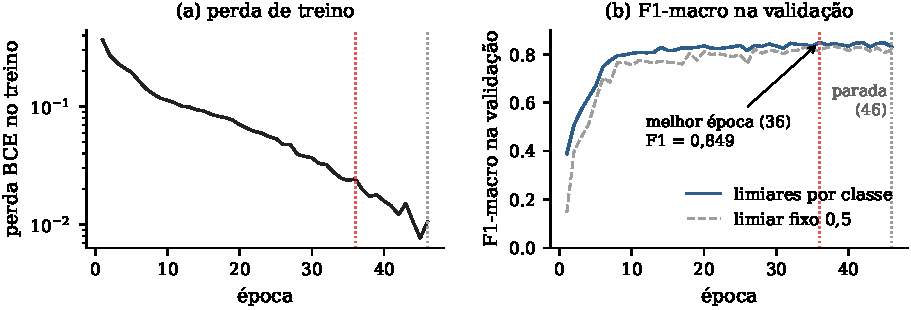
\includegraphics[width=\linewidth]{figs/treino.pdf}
\fonte{Elaborado pelo autor.}
\end{figure}

\paragraph{Limiar de decisão por classe.} A rede devolve uma probabilidade por classe, e é preciso escolher a partir de que valor a classe é considerada presente. O valor 0,5 é a escolha padrão, mas não é necessariamente o melhor para cada classe: em classes raras ou difíceis, as probabilidades dos casos positivos tendem a ser menores, e um limiar mais baixo recupera mais casos; em outras, um limiar mais alto evita falsos positivos. O procedimento adotado, o mesmo do código de Zhang et al.\ (2021), é o seguinte:
\begin{enumerate}
\item ao fim de cada época, calculam-se as probabilidades do modelo para os 1\,378 ECGs da validação;
\item para cada classe, testam-se os limiares de 0,00 a 1,00, em passos de 0,01, e calcula-se o F1 dessa classe na validação com cada um;
\item escolhe-se, para cada classe, o limiar de maior F1 (Figura~\ref{fig:limiar});
\item o F1-macro da validação com esses limiares é o critério da parada antecipada; os nove limiares da melhor época (36) são guardados com o modelo e aplicados, sem mudança, ao conjunto de teste.
\end{enumerate}
Como o teste não participa da escolha, o F1 do teste não é inflado pelo ajuste. Escolher o limiar que maximiza o F1 é um procedimento conhecido para classificadores que devolvem probabilidades (Lipton, Elkan e Naryanaswamy, 2014). Os limiares obtidos foram: SNR 0,89; AF 0,58; IAVB 0,99; BRE 0,85; BRD 0,36; CAP 0,55; CVP 0,84; STD 0,34; STE 0,41. A Figura~\ref{fig:limiar} mostra que o F1 varia pouco numa faixa ampla de limiares (por exemplo, AF entre 0,1 e 0,9), de modo que o valor exato do limiar pesa pouco. O limiar de IAVB é alto (0,99) porque o modelo dá probabilidade acima de 0,5 a 63 ECGs da validação que não têm IAVB; subir o limiar elimina a maior parte desses falsos positivos (18 restam com 0,99) e perde poucos casos verdadeiros (de 134 para 124 dos 144). Entre 0,95 e 0,995, o F1 de IAVB fica praticamente estável (0,86 a 0,87). Lipton, Elkan e Naryanaswamy (2014) mostram que, num classificador com probabilidades bem calibradas, o limiar ótimo seria a metade do F1 ótimo (cerca de 0,43 aqui); um limiar de 0,99 indica que, nessa classe, as probabilidades do modelo são altas demais para ECGs sem IAVB, o que o ajuste do limiar corrige.

\begin{figure}[H]\centering
\caption{F1 na validação em função do limiar de decisão, para três classes. O ponto marca o limiar escolhido; a linha tracejada, o limiar padrão de 0,5.}\label{fig:limiar}
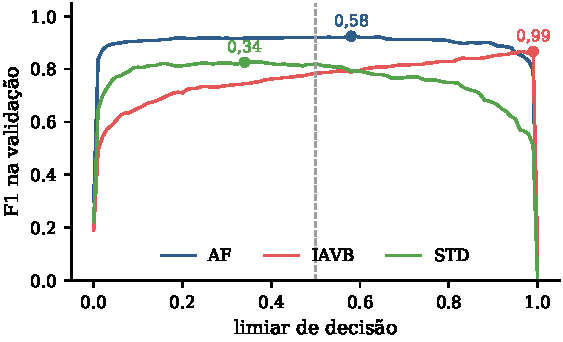
\includegraphics[width=0.62\linewidth]{figs/limiar.pdf}
\fonte{Elaborado pelo autor.}
\end{figure}

\paragraph{Escolha da função de perda.} Como as classes têm frequências muito diferentes (BRD tem 1\,304 registros no treino e STE, 154), foi testada também uma BCE ponderada, que dá aos casos positivos de cada classe um peso igual à razão entre negativos e positivos dessa classe, o que compensa as classes raras. Os dois modelos foram treinados com a mesma configuração, mudando só a perda. Com os limiares por classe, o F1-macro no teste foi de 0,819 com a BCE simples e de 0,816 com a ponderada. A diferença (0,003) é menor do que a variação observada entre dois treinos anteriores com BCE ponderada (0,816 com até 60 épocas e 0,803 com 40 épocas, cerca de 0,01), de modo que as duas perdas são equivalentes nesse critério. Adotou-se a BCE simples por dois motivos. O primeiro é a fidelidade à referência: é a perda usada no código de Zhang et al.\ (2021). O segundo é que ela depende menos do ajuste de limiar: com o limiar fixo de 0,5 para todas as classes, o F1-macro no teste foi de 0,806 com a BCE simples e de 0,785 com a ponderada. Ou seja, o ajuste por classe acrescentou 0,013 ao modelo com BCE simples e 0,031 ao modelo com BCE ponderada: com a ponderação, que aumenta o peso dos casos positivos, o limiar 0,5 fica mais longe do ponto de corte de melhor F1.

% ---------------------------------------------------------------------
\subsection{Explicações GradientSHAP}\label{sec:gshap}

\subsubsection{O que é explicado}
Para cada ECG $x$ e cada classe $c$, o GradientSHAP produz um \textbf{mapa de atribuição} $\phi$ com a mesma dimensão do ECG (12 × 15\,000): um valor para cada derivação e cada instante, que indica quanto aquele ponto contribuiu para o logit $z_c$. Um valor positivo indica que o ponto aumenta a evidência da classe; um negativo, que a diminui. Foram explicadas só as \textbf{predições corretas} do teste: para cada registro, um mapa para cada classe que está presente no registro e foi predita pelo modelo. São \textbf{622 mapas}, distribuídos entre as classes como na Tabela~\ref{tab:f1}. Explicar só os acertos é prática comum na avaliação de explicações em ECG (Suh et al., 2024, usam só predições com probabilidade acima de 0,9; Gumpfer et al., 2026, só verdadeiros positivos), para que a explicação descreva uma decisão correta do modelo. Foi usada a implementação da biblioteca Captum.

\subsubsection{Como o mapa é calculado}
A fundamentação do GradientSHAP está no capítulo de Fundamentação Teórica; aqui se descreve como ele foi configurado. O mapa é a média de $M = 200$ sorteios. Em cada sorteio $m$ (Figura~\ref{fig:gshap}):
\begin{enumerate}
\item \textbf{sorteia-se uma referência} $r_m$ entre 36 ECGs reais do treino (o ``ponto de partida'' com o qual o ECG é comparado);
\item \textbf{soma-se um ruído gaussiano} pequeno ao ECG explicado, $\tilde{x}_m = x + \varepsilon_m$, com $\varepsilon_m \sim \mathcal{N}(0;\,0{,}09^2)$ em cada ponto;
\item \textbf{sorteia-se um ponto no caminho} entre a referência e o ECG, $x'_m = r_m + \alpha_m(\tilde{x}_m - r_m)$, com $\alpha_m$ sorteado entre 0 e 1;
\item calcula-se o \textbf{gradiente} do logit $z_c$ nesse ponto e multiplica-se, ponto a ponto, pela \textbf{diferença entre o ECG e a referência}.
\end{enumerate}
\begin{equation}
\phi(x) \;=\; \frac{1}{M}\sum_{m=1}^{M} \nabla z_c(x'_m) \odot (\tilde{x}_m - r_m).
\label{eq:gshap}
\end{equation}
O produto tem uma leitura intuitiva: um ponto recebe atribuição alta quando a saída é sensível a ele (gradiente grande) \textbf{e} quando ele é diferente da referência (diferença grande). Em média, a soma das atribuições aproxima a diferença entre o logit do ECG explicado e o logit médio das referências (Lundberg e Lee, 2017): o mapa distribui, entre os pontos, quanto o ECG ``se afasta'' das referências na saída da classe $c$.

\begin{figure}[H]\centering
\caption{Um sorteio do GradientSHAP com sinais reais (derivação II, primeiros 2,5 s de um ECG de BRD): (a) ECG explicado; (b) uma das 36 referências; (c) ECG com o ruído gaussiano; (d) ponto do caminho em que o gradiente é calculado; (e) mapa final dessa derivação, média de 200 sorteios (vermelho: atribuição positiva; azul: negativa).}\label{fig:gshap}
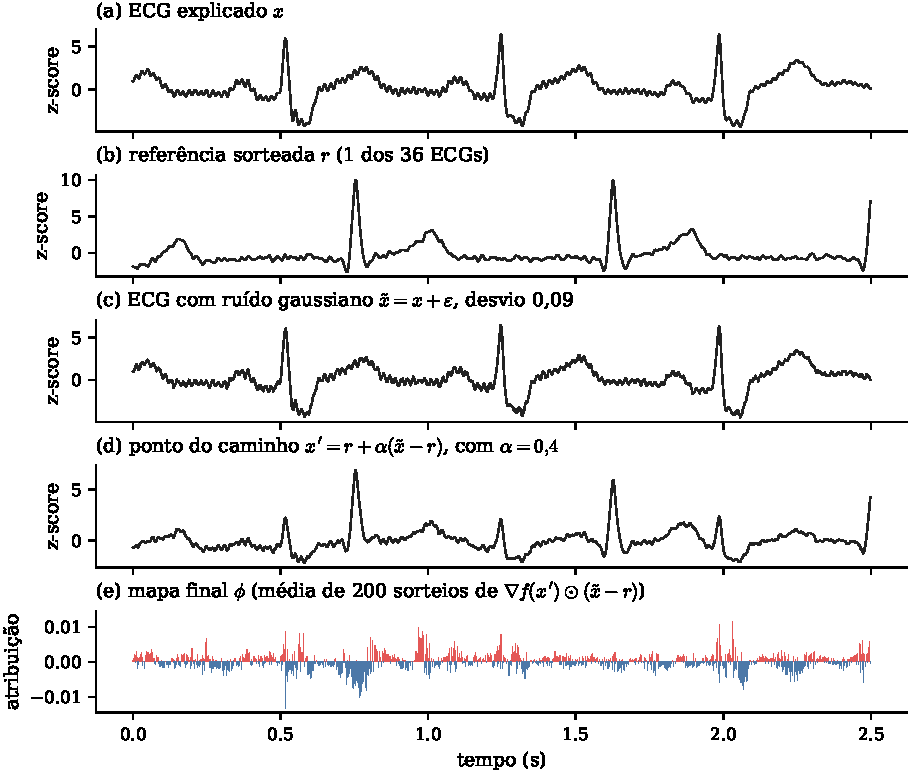
\includegraphics[width=\linewidth]{figs/gshap.pdf}
\fonte{Elaborado pelo autor.}
\end{figure}

\subsubsection{Configuração}
\paragraph{Referência.} As referências são 36 ECGs do treino com um único rótulo, 4 de cada classe, sorteados com semente fixa e usados em todos os mapas. Usar uma \textbf{distribuição} de ECGs reais, em vez de um sinal nulo, segue Turbé et al.\ (2023), que usam 50 ECGs do teste na mesma base: uma linha reta em zero não é um ECG plausível, e o mapa passaria a explicar ``a diferença entre o ECG e uma linha reta''. O balanceamento (4 por classe) evita que a referência represente sobretudo as classes mais comuns, como BRD; com uma referência dominada por uma classe, os ECGs dessa classe ficariam parecidos com a referência e receberiam atribuições artificialmente menores.

\paragraph{Ruído gaussiano.} O ruído do passo 2 faz parte do GradientSHAP e suaviza o mapa: como o gradiente de uma rede ReLU muda de forma abrupta entre pontos vizinhos, a média sobre pequenas variações do ECG reduz oscilações que não refletem o sinal, a mesma ideia do SmoothGrad (Smilkov et al., 2017). O desvio usado, 0,09, é o valor do exemplo de uso do GradientSHAP na documentação da biblioteca Captum; não foi ajustado para o ECG e foi mantido fixo em todo o trabalho. Em unidades de \textit{z-score}, corresponde a 9\% do desvio padrão de cada derivação e a cerca de 0,7\% da amplitude típica de uma derivação (12,9, a mediana entre o máximo e o mínimo nos ECGs de teste), bem abaixo dos 10\% a 20\% da amplitude que Smilkov et al.\ (2017) observam funcionar em imagens. O ruído suaviza, portanto, pouco o mapa (Figura~\ref{fig:gshap}c); a maior parte da suavização vem da média sobre as referências e os pontos do caminho.

\paragraph{Número de sorteios.} Como referência, ruído e $\alpha$ são sorteados, dois mapas do mesmo ECG com sementes diferentes não são iguais. Essa variação é medida pelo \textbf{piso} (seção~\ref{sec:piso}). Com 50 sorteios, o piso médio era de 0,36; com 200, caiu para 0,18 (metade, como esperado para uma média: o erro cai com a raiz do número de sorteios). Optou-se por 200 sorteios, calculados como a média de 4 blocos de 50 (o que cabe na memória da GPU), com uma semente própria para cada mapa. Arends et al.\ (2026) adotam o mesmo cuidado, fixando o número de sorteios para que dois mapas do mesmo ECG tenham correlação de pelo menos 0,98.

% ---------------------------------------------------------------------
\subsection{Regiões do batimento}\label{sec:regioes}

O mapa da seção anterior tem 180\,000 valores (12 × 15\,000). Esta seção descreve como cada mapa é resumido em \textbf{36 valores}, um para cada combinação de derivação (12) e segmento do batimento (pré-QRS, QRS e ST-T), e por que esse resumo é a unidade de todas as métricas.

\subsubsection{Por que agregar os pontos em regiões}
São quatro os motivos.

\paragraph{1. Os pontos isolados não são uma unidade adequada para as métricas.} As versões das métricas na biblioteca Quantus tratam cada um dos 180\,000 valores como um atributo independente, incluindo o preenchimento, que é a maior parte do mapa na maioria dos ECGs (seção~\ref{sec:dados}). Nos testes iniciais deste trabalho, isso gerou resultados sem sentido: a \FC, por exemplo, retirava 224 pontos isolados entre 180\,000 e obtinha correlação próxima de zero, porque retirar pontos esparsos quase não muda a saída do modelo; a \CX\ passava a medir, na prática, a duração do exame.

\paragraph{2. As regiões têm significado clínico.} O diagnóstico de cada classe é descrito pelos cardiologistas em termos de ondas e derivações (por exemplo, ``QRS alargado com padrão rSR' em V1'' no BRD), e não em termos de instantes isolados. Uma região como ``QRS de V1'' é uma unidade que pode ser comparada com esse conhecimento.

\paragraph{3. Somar pontos reduz o ruído do mapa.} Cada sorteio do GradientSHAP usa uma referência, um ruído e um $\alpha$ diferentes (seção~\ref{sec:gshap}). Por isso, o valor do mapa num ponto isolado muda bastante quando o método é repetido com outra semente. Essas flutuações variam de ponto para ponto e, ao somar todos os pontos de uma região, tendem a se cancelar, enquanto a parte comum (a importância real do trecho) se acumula, como na média de várias medidas de uma mesma grandeza. Uma região de QRS, por exemplo, soma 90 amostras em cada batimento e cerca de 1\,400 num ECG de 16 batimentos. Os dados do trabalho mostram o efeito: entre dois mapas do mesmo ECG com sementes diferentes, a distância normalizada (seção~\ref{sec:piso}) é de \textbf{0,53} quando se comparam os 180\,000 pontos e de \textbf{0,18} quando se comparam as 36 regiões. Wagner et al.\ (2024) observam o mesmo efeito ao agregar as atribuições de vários batimentos: a agregação reduz o ruído típico dos métodos de gradiente.

\paragraph{4. Retirar regiões contíguas é uma perturbação mais adequada.} Várias métricas (seção~\ref{sec:metricas}) ``retiram'' partes do ECG e medem a queda da saída. A literatura de séries temporais aponta a falta de agrupamento como um problema dessas métricas (Mercier et al., 2022) e mostra que agrupar pontos consecutivos melhora os seus resultados (Serramazza et al., 2024; Šimić et al., 2025). A diferença fica clara num exemplo: trocar por zero 9 pontos sorteados entre 180\,000 cria 9 ``degraus'' de uma amostra que o modelo nunca viu e que quase não alteram a saída, enquanto trocar por zero o QRS de V1 em todos os batimentos (Figura~\ref{fig:retirada}, seção~\ref{sec:metricas}) remove um componente fisiológico inteiro. Cui et al.\ (2023), em EEG, adotam a mesma solução: perturbam janelas contíguas em vez de pontos sorteados, para introduzir menos ruído de alta frequência no sinal.

\subsubsection{Detecção dos picos R}
As regiões são ancoradas nos picos R, o ponto mais alto do complexo QRS e o ponto mais fácil de detectar com precisão no ECG. Os picos R são detectados na derivação II com a biblioteca NeuroKit2 (filtragem do sinal seguida da detecção de picos, com os parâmetros padrão da biblioteca), como em Gumpfer et al.\ (2026), que usam a mesma biblioteca na derivação I. Como as 12 derivações são registradas ao mesmo tempo, os instantes dos picos R valem para todas elas. Nos 583 ECGs explicados, a mediana é de 16 batimentos completos por ECG (5\% dos ECGs têm 9 ou menos; 5\%, 37 ou mais).

Uma alternativa seria delinear o início e o fim de cada onda (P, QRS e T) batimento a batimento, também com o NeuroKit2. Essa alternativa foi testada e descartada, porque falhou justamente nas classes de interesse: a delineação indicava ``ondas P'' em ECGs de fibrilação atrial, em que não há onda P, e não reconhecia o QRS alargado dos bloqueios de ramo. Janelas definidas a partir do pico R, que é detectado de forma confiável também nesses ECGs, são a solução adotada por trabalhos de avaliação de explicações em ECG: Wagner et al.\ (2024) recortam cada batimento de 300 ms antes a 500 ms depois do pico R para agregar as atribuições, e Turbé et al.\ (2023), na mesma base deste trabalho, de 0,35 s antes a 0,55 s depois para formar o batimento médio.

\subsubsection{Segmentos do batimento}
Cada batimento completo, isto é, o trecho entre dois picos R consecutivos, é dividido em três segmentos (Tabela~\ref{tab:segmentos} e Figura~\ref{fig:regioes}). Os trechos antes do primeiro e depois do último pico R, que não formam um batimento completo, ficam de fora, assim como o preenchimento.

\begin{table}[H]\centering\small
\caption{Segmentos do batimento. $R$ é o instante do pico R e $RR$, o intervalo até o pico R seguinte. As durações da última coluna são para a frequência mediana dos ECGs explicados (77 bpm, $RR \approx 780$ ms).}\label{tab:segmentos}
\begin{tabularx}{\linewidth}{>{\raggedright\arraybackslash}p{2.1cm}>{\raggedright\arraybackslash}p{4.4cm}X>{\raggedleft\arraybackslash}p{1.5cm}}
\toprule
\textbf{Segmento} & \textbf{Intervalo} & \textbf{O que contém} & \textbf{Duração} \\
\midrule
QRS & de $R - 80$ ms a $R + 100$ ms & complexo QRS (despolarização dos ventrículos) & 180 ms \\
ST-T & de $R + 100$ ms a $R + 0{,}45 \cdot RR$ & segmento ST e onda T (repolarização dos ventrículos) & 250 ms \\
pré-QRS & de $R + 0{,}45 \cdot RR$ a 80 ms antes do R seguinte & onda P e intervalo PR (ativação dos átrios e condução até os ventrículos); na AF, as ondas \textit{f} & 350 ms \\
\bottomrule
\end{tabularx}
\fonte{Elaborado pelo autor.}
\end{table}

\begin{figure}[H]\centering
\caption{Segmentos do batimento num ECG de BRD (derivação II): (a) picos R detectados e os três segmentos de cada batimento completo; (b) um batimento ampliado, com os limites usados (linhas contínuas) e os limites alternativos do teste de robustez (tracejadas, seção~\ref{sec:robustez-metodo}).}\label{fig:regioes}
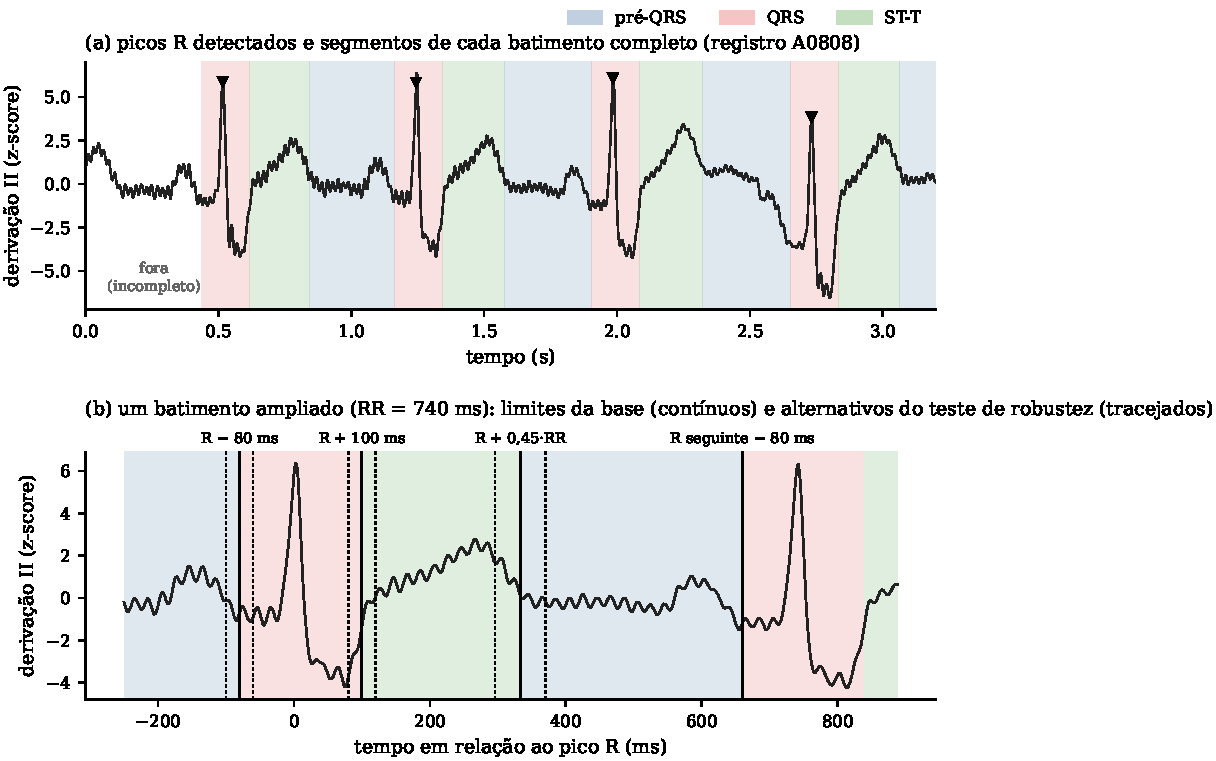
\includegraphics[width=\linewidth]{figs/regioes.pdf}
\fonte{Elaborado pelo autor.}
\end{figure}

\paragraph{Limites do QRS.} A janela do QRS tem 180 ms. O QRS normal dura até cerca de 110 a 120 ms, e o dos bloqueios de ramo completos, duas das classes estudadas, tem 120 ms ou mais (Surawicz et al., 2009)$^{\dagger}$. A janela é assimétrica (80 ms antes e 100 ms depois do pico R) porque, nos bloqueios de ramo, o atraso da condução alonga sobretudo a parte final do QRS, depois do pico R (por exemplo, a onda S larga nas derivações laterais e o R' em V1 no BRD). O limite de 80 ms antes do pico R também é usado como fim do pré-QRS do batimento anterior, de modo que os segmentos não se sobrepõem.

\paragraph{Fim do ST-T.} O fim da onda T não é fixo: o intervalo QT encurta quando a frequência cardíaca aumenta. Por isso, o fim do ST-T é definido como uma fração do intervalo RR de cada batimento, e não em milissegundos. A fração 0,45 vem da fórmula de Bazett, $QT_c = QT/\sqrt{RR}$, a correção do QT mais usada na clínica (Vandenberk et al., 2016), que dá $QT/RR = QT_c/\sqrt{RR}$. A Tabela~\ref{tab:bazett} mostra essa fração para dois valores típicos de $QT_c$ (0,40 e 0,44 s). Com 60 bpm, o QT ocupa de 0,40 a 0,44 do RR; na frequência mediana dos ECGs explicados (77 bpm), de 0,45 a 0,50. A fração 0,45 fica dentro da faixa entre 60 e 77 bpm, que inclui a maioria dos ECGs. Nas frequências altas, a fração cresce, e o final da onda T pode cair no início do pré-QRS. A fórmula de Bazett sobrecorrige o QT em frequências altas (Vandenberk et al., 2016); com a de Fridericia ($QT_c = QT/\sqrt[3]{RR}$), que esse estudo considera mais adequada, as frações são um pouco maiores (Tabela~\ref{tab:bazett}), o que torna o efeito ainda mais provável: nos ECGs explicados, 17\% têm frequência acima de 100 bpm e 7\%, acima de 120 bpm. Esse efeito é avaliado pelo teste de robustez (seção~\ref{sec:robustez-metodo}), que inclui as frações 0,40 e 0,50, e é discutido nas limitações. Uma vantagem de usar a fração do RR é que ela se adapta a cada batimento: numa contração prematura (CAP ou CVP), o RR curto encurta também os segmentos daquele batimento.

\begin{table}[H]\centering\small
\caption{Fração do intervalo RR ocupada pelo QT, pelas fórmulas de Bazett e de Fridericia, para dois valores de QT corrigido.}\label{tab:bazett}
\begin{tabular}{lccccc}
\toprule
\textbf{Frequência (bpm)} & 50 & 60 & 77 (mediana) & 100 & 120 \\
\textbf{RR (ms)} & 1\,200 & 1\,000 & 780 & 600 & 500 \\
\midrule
Bazett, $QT_c = 0{,}40$ s & 0,37 & 0,40 & 0,45 & 0,52 & 0,57 \\
Bazett, $QT_c = 0{,}44$ s & 0,40 & 0,44 & 0,50 & 0,57 & 0,62 \\
Fridericia, $QT_c = 0{,}40$ s & 0,35 & 0,40 & 0,47 & 0,56 & 0,63 \\
Fridericia, $QT_c = 0{,}44$ s & 0,39 & 0,44 & 0,52 & 0,62 & 0,70 \\
\midrule
ECGs explicados nessa faixa & \multicolumn{2}{c}{8\% abaixo de 60} & \multicolumn{1}{c}{metade abaixo de 77} & \multicolumn{2}{c}{17\% acima de 100} \\
\bottomrule
\end{tabular}
\fonte{Elaborado pelo autor.}
\end{table}

\subsubsection{Importância de uma região}
A importância de uma região é a \textbf{soma} do mapa em todos os pontos daquele segmento, em todos os batimentos completos, naquela derivação. Para a derivação $d$ e o segmento $s$:
\begin{equation}
A_{d,s} \;=\; \sum_{b\,\in\,\text{batimentos completos}} \;\; \sum_{t\,\in\,s(b)} \phi_{d,t},
\label{eq:regiao}
\end{equation}
em que $s(b)$ são os instantes do segmento $s$ no batimento $b$. Cada mapa vira, assim, um vetor de 36 valores (12 derivações × 3 segmentos). A Figura~\ref{fig:agregacao} mostra o resultado para o ECG de BRD das figuras anteriores: o mapa de V1, que oscila de ponto a ponto, concentra-se nos QRS, e no vetor das 36 regiões o maior valor é o QRS de V1 (2,8), seguido dos QRS de V2 (1,6) e de V4 (1,2). V1 e V2 são as derivações em que o padrão do BRD (rSR') é reconhecido clinicamente.

\begin{figure}[H]\centering
\caption{Agregação de um mapa em 36 regiões (ECG de BRD): (a) sinal e mapa da derivação V1 nos primeiros 3,2 s, com os segmentos; (b) vetor das 36 regiões do ECG inteiro (10 s), em que cada valor é a soma do mapa naquela derivação e segmento em todos os batimentos completos.}\label{fig:agregacao}
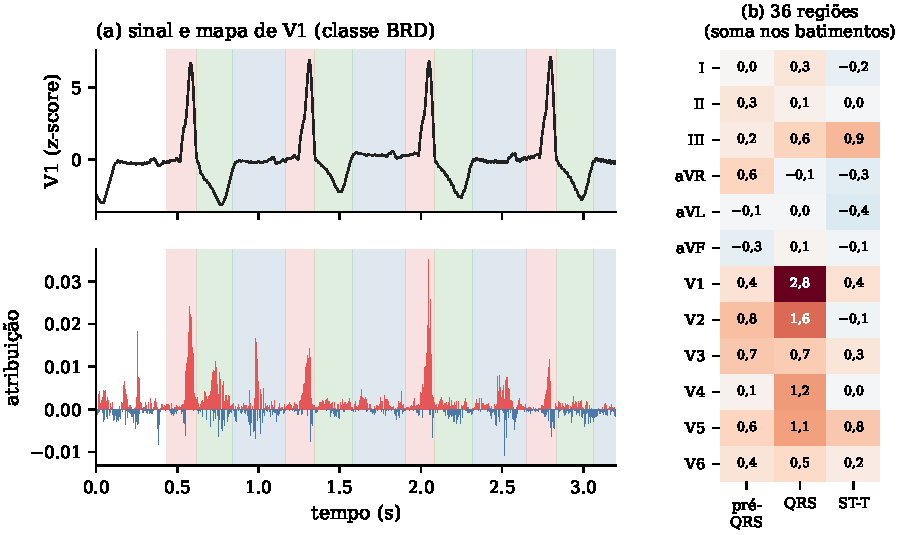
\includegraphics[width=\linewidth]{figs/agregacao.pdf}
\fonte{Elaborado pelo autor.}
\end{figure}

Wagner et al.\ (2024), o precedente mais próximo desse resumo, também organizam as atribuições por derivação e segmento, mas usam a \textbf{média} da atribuição em cada segmento. A soma foi preferida aqui por dois motivos. O primeiro é que Zhang et al.\ (2021), no mesmo modelo e na mesma base, também resumem os valores SHAP pela soma: a contribuição de cada derivação é a soma do mapa em todos os instantes. O segundo é que a soma é coerente com as métricas de retirada: ao retirar uma região, retiram-se todos os seus pontos, e a soma das atribuições é a quantidade que essas métricas comparam com a queda da saída (seção~\ref{sec:metricas}). Com a soma, uma região mais longa pode acumular mais importância só pela duração; o pré-QRS, que é o segmento mais longo (Tabela~\ref{tab:segmentos}), seria o favorecido. Não é o que se observa: no modelo treinado, as duas regiões mais importantes são de QRS, o segmento mais curto, em 42\% dos mapas, e essa fração varia muito entre as classes (seção~\ref{sec:res-emprt}).

O que é próprio deste trabalho é usar essas regiões como \textbf{unidade das métricas}, e não só para visualizar as explicações, calculando-as no registro inteiro (todos os batimentos completos, sem batimento médio) e com as 12 derivações separadas. Gumpfer et al.\ (2026) usam máscaras fixas de PR, QRS e ST, definidas por cardiologistas, para medir se as explicações coincidem com as regiões clínicas; Hicks et al.\ (2021) retiram ondas inteiras (P, QRS ou T) do batimento mediano e medem a piora da predição, uma perturbação por região fisiológica semelhante à usada aqui.

\subsubsection{Robustez dos limites}\label{sec:robustez-metodo}
Os limites dos segmentos são aproximações: outros valores igualmente razoáveis poderiam ter sido escolhidos. Se as conclusões dependessem do valor exato desses limites, seriam frágeis. Para verificar isso, as regiões foram recalculadas com limites alternativos, e as métricas foram recalculadas com as novas regiões, a partir dos mesmos mapas:
\begin{itemize}
\item \textbf{janela do QRS} de 140, 180 (base) ou 220 ms, deslocando cada um dos dois limites em 20 ms (de $R - 60$ a $R + 80$ ms; de $R - 80$ a $R + 100$ ms; de $R - 100$ a $R + 120$ ms);
\item \textbf{fim do ST-T} em 0,40, 0,45 (base) ou 0,50 do RR, o que cobre, pela Tabela~\ref{tab:bazett}, as frequências de 50 a 77 bpm com $QT_c$ de 0,44 s.
\end{itemize}
As 9 combinações (3 × 3) movem os limites em cerca de 2,6\% do batimento na frequência mediana, da mesma ordem do teste de Gumpfer et al.\ (2026), que deslocam as máscaras de PR, QRS e ST em até 10 pontos num batimento de 500 (2\%) e verificam se a ordem dos métodos se mantém. Aqui, o critério é se a \textbf{ordem das classes} se mantém. O teste foi feito nas duas métricas que dependem só do mapa e das regiões, a \CS\ e a \CX\ (seção~\ref{sec:metricas}), e que podem ser recalculadas sem o modelo. As demais exigem passar pelo modelo, para cada combinação, os ECGs com regiões retiradas ou perturbados, o que multiplicaria por nove o custo de GPU dessas métricas, e não foram recalculadas. Os resultados estão na seção~\ref{sec:res-robustez}.

% ---------------------------------------------------------------------
\subsection{O piso: a variação própria do GradientSHAP}\label{sec:piso}

Como o GradientSHAP é estocástico, repetir o cálculo com outra semente dá um mapa um pouco diferente. Isso cria um problema para as métricas que comparam dois mapas: se o mapa de um ECG perturbado é diferente do mapa original, a diferença pode vir da perturbação ou simplesmente do sorteio. O \textbf{piso} é a régua que separa as duas coisas (Figura~\ref{fig:piso}).

\paragraph{Cálculo.} Para cada mapa, gera-se um segundo mapa do mesmo ECG e da mesma classe, com outra semente. Os dois são resumidos nas 36 regiões e normalizados para norma 1 (o vetor é dividido pelo seu comprimento), para que a comparação dependa só do formato do mapa, e não da sua escala. O piso é a distância euclidiana ($\ell_2$) entre os dois vetores. Ele vai de 0 (mapas iguais) a 2 (mapas opostos, com todos os sinais trocados).

\paragraph{Uso.} Três comparações do trabalho são feitas com a \textbf{mesma semente} do mapa original, de modo que os sorteios são idênticos e só muda o que se quer testar: o ECG (\MS\ e \AS), a classe explicada (\RL) ou o modelo (\EM). A distância obtida é lida em relação ao piso do próprio mapa: só uma distância acima do piso indica uma mudança maior do que a do próprio método. A necessidade dessa régua aparece na literatura: o GradientSHAP teve a maior sensibilidade entre os métodos de gradiente nos seis conjuntos de séries temporais de Mercier et al.\ (2022), e Fouladgar et al.\ (2022) observam, em séries temporais, que métodos cujos escores têm escala menor aparecem como menos sensíveis, possivelmente só por causa da escala, o que motiva normalizar os mapas antes de compará-los.

\paragraph{Valores.} O piso médio é de \textbf{0,18}, de 0,13 (BRD e BRE) a 0,25 (CAP).

\begin{figure}[H]\centering
\caption{O piso e o seu uso. Em cima, dois mapas do mesmo ECG e da mesma classe, com sementes diferentes; a distância entre eles é o piso. Embaixo, as três comparações feitas com a mesma semente, em que só muda o ECG, a classe ou o modelo.}\label{fig:piso}
\begin{tikzpicture}[node distance=4mm and 5mm, every node/.style={font=\scriptsize}]
\node[dado] (x) {ECG $x$,\\classe $c$};
\node[proc, right=10mm of x, yshift=6mm] (g1) {GradientSHAP\\semente $s_1$};
\node[proc, right=10mm of x, yshift=-6mm] (g2) {GradientSHAP\\semente $s_2$};
\node[proc, right=of g1] (v1) {36 regiões,\\norma 1};
\node[proc, right=of g2] (v2) {36 regiões,\\norma 1};
\node[saida, right=12mm of v1, yshift=-6mm] (p) {\textbf{piso}\\$\lVert \hat{a}_1 - \hat{a}_2 \rVert_2$\\(média 0,18)};
\draw[seta] (x.east) -- (g1.west); \draw[seta] (x.east) -- (g2.west);
\draw[seta] (g1)--(v1); \draw[seta] (g2)--(v2);
\draw[seta] (v1.east) -- (p.west); \draw[seta] (v2.east) -- (p.west);
% comparações
\node[caixa, below=8mm of g2, xshift=-14mm, align=center] (c1) {\textbf{\MS, \AS}\\ECG perturbado $x + \delta$,\\mesma classe e semente};
\node[caixa, right=of c1, align=center] (c2) {\textbf{\RL}\\mesmo ECG, outra classe $c'$,\\mesma semente};
\node[caixa, right=of c2, align=center] (c3) {\textbf{\EM}\\mesmo ECG, modelo com\\pesos sorteados, mesma semente};
\node[saida, below=6mm of c2, align=center] (l) {distância $d$ ao mapa original (36 regiões, norma 1), lida em relação ao piso do mapa:\\$d$ próximo do piso: a mudança não supera a variação do método;\quad $d$ muito acima do piso: mudança real};
\draw[seta] (c1.south) -- (c1.south |- l.north); \draw[seta] (c2) -- (l); \draw[seta] (c3.south) -- (c3.south |- l.north);
\end{tikzpicture}
\fonte{Elaborado pelo autor.}
\end{figure}

% ---------------------------------------------------------------------
\subsection{Métricas de qualidade das explicações}\label{sec:metricas}

Não há uma única definição de ``boa explicação''. As métricas da literatura medem propriedades diferentes, agrupadas em categorias como fidelidade, robustez, complexidade e randomização, que é a organização da biblioteca Quantus. Foram escolhidas sete métricas, de quatro categorias, para que a pergunta do trabalho fosse respondida para várias propriedades, e não para uma só (Tabela~\ref{tab:metricas}). Os nomes das métricas são mantidos em inglês, como nos artigos de origem e no Quantus, por serem nomes próprios; as categorias são escritas em português.

\begin{table}[H]\centering\small
\caption{Métricas usadas, pergunta que respondem e sentido melhor.}\label{tab:metricas}
\begin{tabularx}{\linewidth}{>{\raggedright\arraybackslash}p{2.1cm}>{\raggedright\arraybackslash}p{3.7cm}X>{\centering\arraybackslash}p{1.4cm}}
\toprule
\textbf{Categoria} & \textbf{Métrica (artigo)} & \textbf{Pergunta} & \textbf{Melhor} \\
\midrule
\multirow{2}{*}{Fidelidade} & \FC\ (Bhatt et al., 2020) & A soma das atribuições de um conjunto de regiões prevê a queda da saída ao retirá-las? & maior \\
 & \FE\ (Alvarez-Melis e Jaakkola, 2018) & A atribuição de cada região prevê a queda ao retirá-la sozinha? & maior \\ \addlinespace
\multirow{2}{*}{Robustez} & \MS, \AS\ (Yeh et al., 2019; Bhatt et al., 2020) & A explicação muda pouco quando o ECG muda pouco? & menor \\
 & \CS\ (Dasgupta et al., 2022) & ECGs com a mesma explicação recebem a mesma predição? & maior \\ \addlinespace
Complexidade & \CX\ (Bhatt et al., 2020) & A importância está concentrada em poucas regiões? & menor \\ \addlinespace
\multirow{2}{*}{Randomização} & \RL\ (Sixt et al., 2020) & O mapa é específico da classe explicada? & maior \\
 & \EM\ (Hedström et al., 2023a) & O mapa depende do que o modelo aprendeu? & maior \\
\bottomrule
\end{tabularx}
\fonte{Elaborado pelo autor.}
\end{table}

Todas as métricas foram \textbf{reimplementadas sobre as 36 regiões}; as versões ponto a ponto do Quantus foram usadas só na fase inicial e descartadas, pelos problemas descritos a seguir em cada métrica. Em cada caso, a implementação segue a definição do artigo original, e as diferenças são só as necessárias para usar regiões no lugar de pontos. A Tabela~\ref{tab:adesao} resume essas diferenças.

\subsubsection{Retirar uma região: o valor de substituição}
As duas métricas de fidelidade ``retiram'' regiões do ECG e medem quanto o logit da classe explicada cai. Retirar uma região é trocar todos os seus pontos, em todos os batimentos, por um valor de referência (Figura~\ref{fig:retirada}). Como o valor escolhido pode carregar informação numa série temporal (Höllig et al., 2023) e mudar os resultados entre classes (Baer et al., 2025a), foram usadas as duas referências propostas por Bhatt et al.\ (2020): \textbf{zero}, que em \textit{z-score} corresponde à média da derivação, e a \textbf{média do treino} em cada derivação e instante. Os resultados com as duas foram iguais até a terceira casa decimal (seção~\ref{sec:res-fidelidade}), e o texto usa a referência zero.

\begin{figure}[H]\centering
\caption{Retirada de uma região: o QRS de V1, em todos os batimentos completos, substituído por zero (a média da derivação).}\label{fig:retirada}
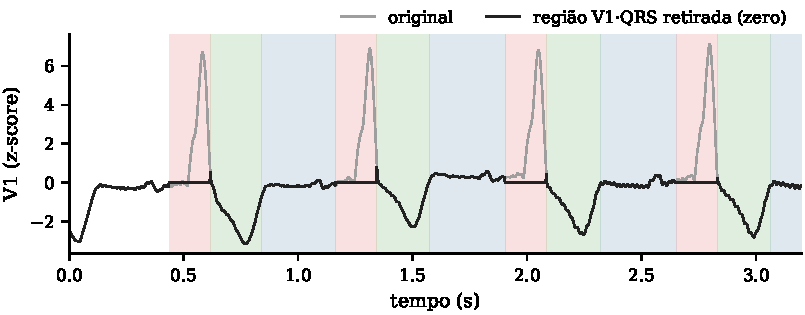
\includegraphics[width=\linewidth]{figs/retirada.pdf}
\fonte{Elaborado pelo autor.}
\end{figure}

\subsubsection{Fidelidade: \FC\ e \FE}
\paragraph{Definição original.} A \FC\ (Bhatt et al., 2020, Definição 3) sorteia subconjuntos $S$ de atributos de um exemplo, retira cada subconjunto e calcula a correlação de Pearson, entre os subconjuntos, da soma das atribuições de $S$ com a queda da saída $f(x) - f(x_{[S = \text{ref}]})$. A \FE\ (Alvarez-Melis e Jaakkola, 2018, seção 5.3) retira cada atributo isoladamente e correlaciona a sua atribuição com a queda. Se as atribuições são fiéis, as regiões mais importantes são as que mais derrubam a saída quando retiradas.

\paragraph{Implementação.} Os atributos são as 36 regiões. Na \FC, para cada mapa, são sorteados 50 subconjuntos de 9 regiões (um quarto das 36), e a análise foi repetida com 4 e 18 regiões. Na \FE, cada uma das 36 regiões é retirada uma vez. Em ambas, a saída é o logit da classe explicada, e a correlação é calculada para cada mapa e depois resumida pela média de cada classe. Na \FE, a probabilidade, que é a saída do artigo original, foi calculada como verificação; o logit foi preferido porque a probabilidade satura perto de 1 nos ECGs classificados com alta confiança, e a queda deixa de ser visível.

\paragraph{Por que não a versão do Quantus.} Na configuração padrão, a \FC\ do Quantus retira 224 pontos isolados, trocados pelo mínimo do próprio sinal, e a \FE\ retira grupos de 500 pontos em ordem de atribuição; nos dois casos, a queda medida refletia o dano causado ao sinal por valores extremos, e não a retirada de informação, e a \FC\ resultou próxima de zero. O cálculo por regiões mantém a definição dos artigos e muda só o que é um atributo.

\subsubsection{Robustez: \MS, \AS\ e \CS}
\paragraph{Definição original.} A \MS\ (Yeh et al., 2019, Definição 3.1) é a maior mudança da explicação quando o exemplo é perturbado dentro de uma vizinhança de raio $r$; a \AS\ (Bhatt et al., 2020, Definição 2) é a mudança média. A \CS\ (Dasgupta et al., 2022, Definição 1) parte de outra ideia: exemplos que recebem a mesma explicação devem receber a mesma predição. Como explicações contínuas quase nunca são idênticas, elas são primeiro discretizadas; o artigo usa o sinal dos 5 atributos mais importantes (Apêndice D.5) e estima a métrica, para cada exemplo, como a fração dos outros exemplos com a mesma explicação discretizada que têm a mesma predição (seção 4.1).

\paragraph{Implementação das sensibilidades.} Para cada mapa, são feitas 10 perturbações: a cada ponto do trecho real do ECG soma-se um ruído uniforme entre $-0{,}1$ e $0{,}1$ (10\% do desvio padrão da derivação), sem tocar no preenchimento. Cada ECG perturbado é explicado com a mesma semente do mapa original, para que a diferença reflita só a perturbação (seção~\ref{sec:piso}). Perturbações que tiram a classe da predição são descartadas, como em Bhatt et al.\ (2020), porque nesse caso é esperado que a explicação mude. A mudança é a distância $\ell_2$ entre os vetores das 36 regiões normalizados; a \MS\ é a maior das 10 distâncias e a \AS, a média. As duas são comparadas com o piso. A versão do Quantus comparava o mapa salvo com mapas refeitos com outro número de sorteios e outra semente, perturbava também o preenchimento e não descartava as perturbações que mudam a predição; com isso, a variação do próprio método se confundia com a sensibilidade.

\paragraph{Implementação da \CS.} Cada mapa é discretizado como as 2 regiões de maior $|A_{d,s}|$, com o sinal de cada uma (por exemplo, ``QRS de V1 positivo e QRS de V2 positivo''). Com 36 regiões, a discretização do artigo, com 5 atributos, tornaria quase todas as explicações únicas, e a métrica perderia o sentido. A análise foi repetida com 1 e 3 regiões (seção~\ref{sec:res-consistency}). A predição de cada mapa é a classe que ele explica, e os 622 mapas formam uma única população. Como a métrica depende de quantos mapas cada classe tem (classes com muitos mapas têm mais chance de coincidir), calcula-se também o valor esperado ao acaso, mantendo as explicações e embaralhando as classes entre os mapas. A discretização padrão do Quantus (sinal dos 5 primeiros valores do mapa) atribuía a mesma explicação a todos os mapas, porque os primeiros pontos de um ECG não dizem nada sobre o diagnóstico.

\subsubsection{Complexidade: \CX}
\paragraph{Definição original e implementação.} A \CX\ (Bhatt et al., 2020, Definição 4) é a entropia das frações de importância, $H = -\sum_i P_i \ln P_i$, com $P_i = |A_i| / \sum_j |A_j|$. Uma explicação concentrada em poucos atributos é mais fácil de interpretar e tem entropia baixa. Aqui, os atributos são as 36 regiões. Para facilitar a leitura, a entropia é convertida no \textbf{número efetivo de regiões}, $e^{H}$: o número de regiões que, com a mesma importância cada uma, dariam a mesma entropia. Ele vai de 1 (tudo numa região) a 36 (importância igual em todas). O índice de Gini das importâncias (a \textit{Sparseness} do Quantus) foi calculado como verificação. No Quantus, a métrica usa os 180\,000 pontos, inclusive o preenchimento, e passa a depender da duração do exame.

\subsubsection{Randomização: \RL\ e \EM}
\paragraph{Definição original.} O \RL\ (Sixt et al., 2020, seção 3) compara o mapa da classe explicada com o mapa de outra classe no mesmo exemplo: se forem quase iguais, a explicação não é específica da classe. O \EM\ (Hedström et al., 2023a, Definição 3) compara o mapa do modelo treinado ($e$) com o mapa de um modelo com todos os pesos sorteados de novo ($\hat{e}$), pelo aumento relativo da complexidade, $q = (\xi(\hat{e}) - \xi(e))/\xi(e)$, em que $\xi$ é a entropia do mapa: se o mapa descreve o que o modelo aprendeu, o modelo aleatório deve dar um mapa mais espalhado, e $q > 0$.

\paragraph{Implementação do \RL.} No mesmo ECG, geram-se os mapas das 8 outras classes, com a mesma semente, e calcula-se a distância $\ell_2$ normalizada nas 36 regiões entre cada um e o mapa da classe explicada. O resultado principal usa as classes \textbf{ausentes} do ECG; as presentes, em ECGs com mais de um diagnóstico, são registradas à parte, porque podem usar legitimamente a mesma evidência. A distância é comparada com o piso. O Quantus sorteia a outra classe sem distinguir presentes de ausentes, gera o novo mapa com outros sorteios (misturando a variação do método com a da classe) e mede a semelhança pelo SSIM, uma medida feita para imagens, sobre os 180\,000 pontos.

\paragraph{Implementação do \EM.} Os pesos de todas as camadas da ResNet são sorteados de novo, com 3 sementes, e o mapa de cada ECG é refeito com a mesma semente e a mesma referência do mapa original, de modo que só o modelo muda. A entropia $\xi$ é a das 36 regiões, a mesma da \CX. O artigo calcula $\xi$ por um histograma dos valores do mapa; essa versão foi calculada como verificação em 174 mapas. Como complemento, são registradas a distância entre os dois mapas, com e sem o sinal das atribuições, comparada com o piso, e a fração de mapas com as 2 regiões principais no QRS.

\begin{table}[H]\centering\small
\caption{Aderência das implementações aos artigos originais.}\label{tab:adesao}
\begin{tabularx}{\linewidth}{>{\raggedright\arraybackslash}p{2.5cm}>{\raggedright\arraybackslash}p{4.6cm}X}
\toprule
\textbf{Métrica} & \textbf{Mantido do artigo} & \textbf{Adaptado no TCC (e por quê)} \\
\midrule
\FC & subconjuntos sorteados; Pearson entre soma das atribuições e queda; referências zero e média & atributo = região; logit como saída; $|S| = 9$ (também 4 e 18) \\ \addlinespace
\FE & cada atributo retirado sozinho; Pearson & atributo = região; logit como saída (probabilidade satura), probabilidade como verificação \\ \addlinespace
\MS, \AS & máximo e média da mudança numa vizinhança $\ell_\infty$; distância entre mapas normalizados; descarte das perturbações que mudam a predição & distância nas 36 regiões; mesma semente; leitura em relação ao piso (método estocástico) \\ \addlinespace
\CS & estimador da seção 4.1; discretização pelo sinal dos atributos principais & 2 regiões em vez de 5 atributos (também 1 e 3); valor ao acaso como referência \\ \addlinespace
\CX & entropia das frações de importância & atributo = região; leitura como número efetivo $e^H$; Gini como verificação \\ \addlinespace
\RL & mapa da classe explicada × mapa de outra classe & distância $\ell_2$ em vez de SSIM; classes ausentes × presentes; mesma semente; piso \\ \addlinespace
\EM & todas as camadas randomizadas; $q$ como aumento relativo da entropia & entropia nas regiões (histograma como verificação); 3 sementes; distâncias e fração no QRS como complemento \\
\bottomrule
\end{tabularx}
\fonte{Elaborado pelo autor.}
\end{table}

Não se encontrou, na revisão da literatura, aplicação em ECG das sete métricas em conjunto, nem o cálculo por regiões fisiológicas lido em relação à variação do método. Partes do conjunto têm precedentes: a \FC\ foi aplicada a ECG por Suh et al.\ (2024), ponto a ponto e com substituição por zero, e \FC, \MS, \AS\ e \CX\ foram usadas juntas em séries temporais pelo XTSC-Bench (Höllig et al., 2023).

% ---------------------------------------------------------------------
\subsection{Forma de análise}\label{sec:analise}
Para cada métrica, calcula-se a média dos mapas de cada classe, e as nove classes são ordenadas da melhor para a pior. Essa ordem é comparada com a ordem das classes pelo F1 no teste, com atenção especial às pontas: as três classes de maior F1 (AF, BRD e IAVB) e as duas de menor (CAP e STE). A comparação é \textbf{descritiva}. Não se calculam correlações entre as métricas e o F1 porque há só nove classes, que não são uma amostra independente de uma população: com $n = 9$, uma correlação de postos precisaria de $|\rho| \ge 0{,}70$ para ser distinguível do acaso, e uma classe a mais ou a menos mudaria a conclusão. Arends et al.\ (2026) também tratam a relação com o desempenho por classe de forma descritiva. Os fatores, além do desempenho, que podem ordenar as classes em cada métrica são discutidos junto com os resultados (seção~\ref{sec:sintese}).

\subsection{Ambiente computacional}
O treino do modelo, a geração dos mapas e as métricas que precisam do modelo (fidelidade, sensibilidade, \RL\ e \EM) foram executados no Kaggle, com GPU NVIDIA T4. A \CS, a \CX, o teste de robustez dos limites e as figuras foram calculados localmente, na CPU. O código foi escrito em Python, com PyTorch para o modelo, Captum 0.9 para o GradientSHAP, NeuroKit2 0.2 para a detecção dos picos R e NumPy, SciPy e Matplotlib para a análise; todo o código e os resultados estão no repositório do trabalho.

% =====================================================================
\section{Resultados e Discussão}\label{sec:resultados}

Este capítulo apresenta, primeiro, o desempenho do classificador, que é a referência das comparações (seção~\ref{sec:res-f1}). Em seguida, apresenta os resultados de cada métrica e os discute à luz da literatura (seções~\ref{sec:res-visao} a~\ref{sec:res-emprt}), verifica a robustez dos resultados à definição das regiões (seção~\ref{sec:res-robustez}) e, por fim, reúne o que as métricas dizem sobre a relação com o F1 (seção~\ref{sec:sintese}) e as limitações do trabalho (seção~\ref{sec:limitacoes}).

\subsection{Desempenho do classificador}\label{sec:res-f1}
O modelo obteve F1-macro de \textbf{0,819} no teste, próximo do relatado por Zhang et al.\ (2021) na mesma base e com a mesma arquitetura (0,813, média de 10 dobras). A Tabela~\ref{tab:f1} traz o F1 por classe, ordenado do maior para o menor, e o número de mapas explicados de cada classe. A ordem admite uma leitura clínica: as classes de maior F1 têm sinais claros e extensos no traçado, como a irregularidade do ritmo na AF, o QRS alargado no BRD e o PR longo no IAVB; as de menor F1 dependem de alterações pequenas ou de um único batimento, como a onda P precoce na CAP e o desvio do segmento ST na STE, que é também a classe com menos exemplos (154 no treino e 22 no teste). O F1 por classe também é próximo do de Zhang et al.\ (2021): a maior diferença é de 0,06 (STE, 0,596 contra 0,535), e as classes melhores (AF e BRD, acima de 0,9) e a pior (STE) coincidem. Zhang et al.\ atribuem o F1 baixo de STE à grande discordância entre médicos no diagnóstico dessa classe. Como a avaliação aqui usa uma única divisão, e a de Zhang et al., a média de 10 dobras, os números não são diretamente equivalentes. Essa ordem é a referência das comparações deste capítulo.

\begin{table}[H]\centering\small
\caption{F1 por classe no teste, com os limiares por classe e com o limiar fixo de 0,5, F1 relatado por Zhang et al.\ (2021) e número de mapas explicados (predições corretas). Classes ordenadas pelo F1 deste trabalho.}\label{tab:f1}
\setlength{\tabcolsep}{4.5pt}
\begin{tabular}{lrrrrrrrrr|r}
\toprule
& AF & BRD & IAVB & BRE & CVP & SNR & STD & CAP & STE & Macro \\
\midrule
F1 (limiares por classe) & 0,931 & 0,927 & 0,884 & 0,870 & 0,837 & 0,796 & 0,778 & 0,750 & 0,596 & 0,819 \\
F1 (limiar 0,5) & 0,931 & 0,921 & 0,811 & 0,857 & 0,814 & 0,772 & 0,778 & 0,750 & 0,622 & 0,806 \\
F1, Zhang et al.\ (2021)\textsuperscript{a} & 0,919 & 0,926 & 0,864 & 0,866 & 0,851 & 0,805 & 0,814 & 0,735 & 0,535 & 0,813 \\
Mapas explicados & 108 & 172 & 61 & 20 & 59 & 78 & 65 & 45 & 14 & 622 \\
\bottomrule
\end{tabular}
\fonte{Dados do presente estudo; \textsuperscript{a}Zhang et al.\ (2021), Tabela II, média de 10 dobras.}
\end{table}

\subsection{Visão geral das métricas por classe}\label{sec:res-visao}
A Tabela~\ref{tab:res} traz o valor de cada métrica por classe e a Tabela~\ref{tab:ordens}, a ordem das classes em cada uma. Nenhuma métrica reproduz exatamente a ordem do F1, mas algumas se aproximam dela nas pontas e outras seguem um padrão diferente, que é o assunto das seções seguintes.

\begin{table}[H]\centering\small
\caption{Métricas por classe. Classes na ordem do F1. FC: \FC\ ($|S| = 9$, referência zero). FE: \FE\ (logit, referência zero). Max-S: \MS. N.º efet.: número efetivo de regiões (\CX). Cons.: \CS\ (entre parênteses, o valor ao acaso). RL: distância do \RL\ às classes ausentes. Setas: sentido melhor.}\label{tab:res}
\setlength{\tabcolsep}{4pt}
\begin{tabular}{lrrrrrrrr}
\toprule
\textbf{Classe} & \textbf{F1} & \textbf{FC} $\uparrow$ & \textbf{FE} $\uparrow$ & \textbf{Max-S} $\downarrow$ & \textbf{Piso} & \textbf{N.º efet.} $\downarrow$ & \textbf{Cons.} $\uparrow$ & \textbf{RL} $\uparrow$ \\
\midrule
AF   & 0,931 & 0,544 & 0,515 & 0,056 & 0,19 & 22,9 & 0,457 (0,145) & 1,687 \\
BRD  & 0,927 & 0,746 & 0,784 & 0,029 & 0,13 & 22,2 & 0,723 (0,231) & 1,632 \\
IAVB & 0,884 & 0,647 & 0,553 & 0,041 & 0,18 & 23,0 & 0,424 (0,081) & 1,607 \\
BRE  & 0,870 & 0,651 & 0,698 & 0,033 & 0,13 & 26,2 & 0,335 (0,026) & 1,622 \\
CVP  & 0,837 & 0,618 & 0,659 & 0,047 & 0,17 & 25,0 & 0,382 (0,078) & 1,626 \\
SNR  & 0,796 & 0,448 & 0,493 & 0,049 & 0,23 & 26,2 & 0,260 (0,104) & 1,479 \\
STD  & 0,778 & 0,471 & 0,491 & 0,056 & 0,23 & 26,9 & 0,389 (0,086) & 1,483 \\
CAP  & 0,750 & 0,503 & 0,544 & 0,066 & 0,25 & 25,4 & 0,163 (0,059) & 1,578 \\
STE  & 0,596 & 0,633 & 0,592 & 0,045 & 0,18 & 25,5 & 0,084 (0,018) & 1,426 \\
\midrule
Global & 0,819 & 0,600 & 0,611 & 0,045 & 0,18 & 24,1 & 0,455 & 1,595 \\
\bottomrule
\end{tabular}
\fonte{Dados do presente estudo.}
\end{table}

\begin{table}[H]\centering\small
\caption{Ordem das classes em cada métrica, da melhor para a pior.}\label{tab:ordens}
\begin{tabular}{lccccccccc}
\toprule
\textbf{Critério} & \textbf{1.º} & \textbf{2.º} & \textbf{3.º} & \textbf{4.º} & \textbf{5.º} & \textbf{6.º} & \textbf{7.º} & \textbf{8.º} & \textbf{9.º} \\
\midrule
F1 & AF & BRD & IAVB & BRE & CVP & SNR & STD & CAP & STE \\
\midrule
\CS & BRD & AF & IAVB & STD & CVP & BRE & SNR & CAP & STE \\
\RL & AF & BRD & CVP & BRE & IAVB & CAP & STD & SNR & STE \\
\FC & BRD & BRE & IAVB & STE & CVP & AF & CAP & STD & SNR \\
\FE & BRD & BRE & CVP & STE & IAVB & CAP & AF & SNR & STD \\
\MS & BRD & BRE & IAVB & STE & CVP & SNR & AF & STD & CAP \\
\CX\ (concentração) & BRD & AF & IAVB & CVP & CAP & STE & SNR & BRE & STD \\
\bottomrule
\end{tabular}
\fonte{Dados do presente estudo.}
\end{table}

\subsection{Fidelidade}\label{sec:res-fidelidade}
A \FC\ global é de 0,60 e a \FE, de 0,61: a soma das atribuições prevê de forma moderada a queda da saída quando as regiões são retiradas. Os valores são próximos dos da literatura. Suh et al.\ (2024), em cinco bases de ECG, obtiveram para o DeepSHAP, da mesma família do GradientSHAP, \FC\ de 0,41 a 0,63, a maior entre os 11 métodos avaliados, calculada ponto a ponto. Correlações moderadas, e não próximas de 1, também são esperadas por Turbé et al.\ (2023), que, na mesma base, concluem que a relevância atribuída pelos métodos funciona mais como uma \textbf{ordem} de importância do que como uma contribuição proporcional. O resultado não dependeu do valor de substituição (zero e média do treino deram a mesma \FC, 0,600) e foi parecido com 4 e 18 regiões por subconjunto (0,606 e 0,547).

\paragraph{Frente ao F1.} A fidelidade \textbf{não} acompanha o F1 nas pontas. BRD está no topo das duas métricas (0,75 e 0,78) e também no topo do F1, mas AF, a classe de maior F1, é só a 6.ª na \FC\ e a 7.ª na \FE; STE, a de menor F1, é a 4.ª nas duas. A ordem segue outro padrão: as classes reconhecidas pela \textbf{forma do QRS} (BRD, BRE e CVP) ficam no alto; as de \textbf{ritmo e onda P} (SNR, AF e CAP) e a de \textbf{depressão de ST} (STD), embaixo. O padrão se repete com 4, 9 e 18 regiões por subconjunto: BRD é a primeira e STD e SNR, as duas últimas, nos três casos.

\paragraph{Relação com a literatura.} Esse padrão concorda com Gumpfer et al.\ (2026), que compararam as explicações com regiões definidas por diretrizes clínicas no PTB-XL: o GradientSHAP cobre bem o QRS nos bloqueios de ramo e fica abaixo do acaso no segmento ST da isquemia, porque métodos que multiplicam o gradiente pela entrada, ou subtraem uma referência, concentram a atribuição nos componentes de grande amplitude. O QRS é o componente de maior amplitude do ECG; o segmento ST, a onda P e a irregularidade do ritmo são desvios pequenos ou distribuídos no tempo. Baer et al.\ (2025b) mostram, com dados sintéticos de evidência conhecida, que diferenças simples de amplitude ou de duração do padrão entre as classes bastam para mudar as métricas de perturbação, a ponto de ordenar as classes ao contrário da verdade. Por isso, a diferença de fidelidade entre as classes não deve ser lida, por si, como diferença de qualidade das explicações, como recomendam Baer et al.\ (2025a). A AF ilustra o caso: a evidência da classe está na irregularidade dos intervalos RR, que é uma propriedade da sequência de batimentos, e não de uma região isolada; retirar uma região não retira essa evidência, e a queda da saída deixa de acompanhar a atribuição. A posição de STE, com só 14 mapas, deve ser lida com cautela.

\subsection{Robustez}\label{sec:res-robustez-sens}
A \MS\ global é de 0,045 e a \AS, de 0,036, ambas cerca de quatro vezes \textbf{menores que o piso} (0,18). Ou seja, uma perturbação pequena do ECG muda a explicação menos do que repetir o próprio GradientSHAP com outra semente. Ao passar de 50 para 200 sorteios, a \MS\ caiu cerca de 40\% (de 0,072 para 0,045): parte da sensibilidade medida com 50 sorteios era erro de estimativa do próprio método. Isso concorda com Mercier et al.\ (2022), em que o GradientSHAP teve a maior sensibilidade entre os métodos de gradiente, e mostra por que a leitura em relação ao piso é necessária: sem ela, a variação do método seria interpretada como falta de robustez da explicação.

\paragraph{Frente ao F1.} A ordem das classes repete a da fidelidade, e não a do F1: BRD e BRE são as mais robustas; CAP, STD e AF, as menos. As classes menos robustas são também as de piso mais alto (CAP 0,25; STD e SNR 0,23), ou seja, aquelas em que o próprio GradientSHAP é menos estável. Uma explicação plausível, coerente com a seção anterior, é que nas classes de QRS a atribuição se concentra num componente de grande amplitude, que domina o mapa em qualquer sorteio, enquanto nas de evidência pequena ou distribuída o mapa depende mais da referência e do ruído sorteados.

\subsection{Complexidade}\label{sec:res-complexidade}
Os mapas usam, em média, o equivalente a \textbf{24 das 36 regiões}: a importância é espalhada, e não concentrada em poucas regiões. BRD, AF e IAVB têm os mapas mais concentrados (22 a 23 regiões); STD, SNR e BRE, os mais espalhados (26 a 27). Reduzir o erro de estimativa, de 50 para 200 sorteios, quase não mudou a complexidade (de 24,2 para 24,1): o espalhamento vem do modelo, e não do ruído do método. Também não é uma escolha de unidade: a Figura~\ref{fig:agregacao} mostra um mapa de BRD com uma região claramente dominante (QRS de V1) e, ainda assim, valores não nulos em quase todas as outras.

\paragraph{Frente ao F1.} As três classes mais concentradas coincidem com as três de maior F1, mas BRE, 4.ª no F1, está entre as mais espalhadas, e CAP e STE, as duas piores no F1, estão no meio. A relação é, portanto, parcial. A complexidade é também a categoria de métricas menos confiável na meta-avaliação de Hedström et al.\ (2023b), o MetaQuantus, o que recomenda não apoiar conclusões só nela.

\subsection{\CS}\label{sec:res-consistency}
A \CS\ global é de 0,455, acima do valor esperado ao acaso em todas as classes (Tabela~\ref{tab:res}). É a métrica cuja ordenação das classes \textbf{mais se aproxima da ordenação pelo F1}: as três classes de maior F1 (AF, BRD e IAVB) são as três de maior \CS, e as duas de menor F1 (CAP e STE) são as duas de menor \CS. Com 1 e 3 regiões na discretização, a ordem muda no meio, mas as pontas se mantêm: BRD em 1.º e CAP e STE nas duas últimas posições.

\paragraph{Ressalvas.} Duas propriedades da métrica a aproximam do desempenho por construção. A primeira é que ela depende da frequência da classe entre os mapas: BRD tem 172 mapas e o maior valor ao acaso (0,23), enquanto STE tem 14 e valor ao acaso de 0,02; por isso, o valor de cada classe deve ser lido junto com o seu valor ao acaso. A segunda é que ela usa as predições do próprio modelo: uma classe que o modelo reconhece por um padrão estável tende a produzir explicações repetidas, e o mesmo padrão estável favorece o F1. A \CS\ responde, assim, a uma pergunta diferente das métricas de fidelidade: não se a explicação reflete o efeito das regiões sobre a saída, mas se explicações iguais correspondem a decisões iguais.

\subsection{Especificidade da classe (\RL)}\label{sec:res-rlogit}
No mesmo ECG, o mapa da classe explicada fica, em média, a \textbf{1,60} do mapa de uma classe ausente (a distância máxima possível é 2), em média \textbf{10 vezes o piso} do próprio mapa, e todos os 4\,886 pares ficam acima do piso do próprio mapa: as explicações são específicas da classe. As pontas acompanham o F1: AF (maior F1) tem as explicações mais específicas e STE (menor F1), as menos; as cinco classes de maior F1 ocupam as cinco primeiras posições, embora em outra ordem entre si.

\paragraph{Relação com a literatura.} Sixt et al.\ (2020) propõem o teste por mostrarem que alguns métodos de explicação produzem quase o mesmo mapa para qualquer classe; não é o caso aqui. O resultado também concorda com Sujatha Ravindran e Contreras-Vidal (2023), em que métodos da família gradiente × entrada foram sensíveis à classe e ao modelo em EEG simulado. O fato de as classes de menor F1 terem as explicações menos específicas é coerente com um modelo que separa pior essas classes das demais: se a evidência que o modelo usa para STE é parecida com a que usa para outras classes, os mapas também ficam parecidos.

\subsection{Dependência do modelo (\EM)}\label{sec:res-emprt}
Com os pesos sorteados de novo, o mapa \textbf{não} fica mais espalhado: o número efetivo de regiões passa de 24,1 para 22,9, e o aumento relativo da entropia é $q = -0{,}015$, com só 37\% dos mapas com $q > 0$. Com a entropia de histograma do artigo, na verificação com 174 mapas, $q = -0{,}31$. Pelo critério de Hedström et al.\ (2023a), o GradientSHAP não passa no teste.

Os complementos mostram, porém, que o mapa depende do modelo. A distância entre o mapa do modelo treinado e o do modelo aleatório é \textbf{8,7 vezes o piso} com o sinal das atribuições e 5,8 vezes só com as magnitudes, em todos os 622 mapas, e a região principal coincide em só 5\% dos casos. O critério falha por outro motivo: sem o que o modelo aprendeu, o fator (ECG $-$ referência) da Equação~\ref{eq:gshap} concentra o mapa nos picos do QRS, e um mapa concentrado tem entropia baixa. No modelo aleatório, 88\% dos mapas têm as 2 regiões principais no QRS; no treinado, 42\%. No modelo treinado, essa fração depende da classe (95\% em BRE e 71\% em BRD, contra 2\% em IAVB e 6\% em STD); no aleatório, não.

\paragraph{Relação com a literatura.} Esse comportamento é o previsto por Adebayo et al.\ (2018) para métodos do tipo entrada × gradiente, cujo mapa tende a reproduzir a própria entrada quando o modelo não carrega informação, e concorda com o viés de amplitude descrito por Gumpfer et al.\ (2026) e por Wagner et al.\ (2024), em cujo teste de sanidade os métodos de gradiente × entrada puseram a relevância no pico R mesmo em tarefas sobre as ondas P e T. Arends et al.\ (2026), com ResNet-1D em ECG de 12 derivações, observam correlação próxima de zero entre os mapas antes e depois de randomizar os pesos, o que concorda com as distâncias muito acima do piso obtidas aqui. O \EM\ é usado, por isso, como teste de sanidade do método, e não como métrica de comparação entre classes: a entropia não é um bom critério para métodos cujo mapa no modelo aleatório é concentrado pela própria entrada.

\subsection{Robustez à definição das regiões}\label{sec:res-robustez}
A Tabela~\ref{tab:robreg} mostra a \CS\ e a \CX\ recalculadas nas 9 combinações de limites descritas na seção~\ref{sec:robustez-metodo}. Cada linha é uma definição diferente das regiões, aplicada aos mesmos 622 mapas.

\begin{table}[H]\centering\small
\caption{\CS\ ($k = 2$) e \CX\ (número efetivo de regiões) com limites alternativos das regiões. Em destaque, a definição usada no trabalho. As colunas de ordem trazem as classes da melhor para a pior.}\label{tab:robreg}
\footnotesize\setlength{\tabcolsep}{3pt}
\begin{tabular}{ccc>{\raggedright\arraybackslash}p{4.45cm}c>{\raggedright\arraybackslash}p{4.45cm}}
\toprule
\textbf{QRS} & \textbf{ST-T até} & \textbf{\CS} & \textbf{Ordem na \CS} & \textbf{N.º ef.} & \textbf{Ordem na \CX\ (concentração)} \\
\midrule
140 ms & 0,40 RR & 0,458 & BRD AF STD IAVB CVP SNR BRE CAP STE & 24,1 & IAVB AF BRD CAP STE CVP SNR BRE STD \\
140 ms & 0,45 RR & 0,469 & BRD STD AF IAVB CVP BRE SNR CAP STE & 24,3 & IAVB BRD AF CVP CAP STE SNR BRE STD \\
140 ms & 0,50 RR & 0,467 & BRD STD IAVB AF CVP BRE SNR STE CAP & 24,5 & BRD IAVB AF CVP CAP STE SNR BRE STD \\
180 ms & 0,40 RR & 0,441 & BRD AF IAVB STD CVP BRE SNR CAP STE & 23,8 & BRD AF IAVB CVP CAP STE BRE SNR STD \\
\textbf{180 ms} & \textbf{0,45 RR} & \textbf{0,455} & \textbf{BRD AF IAVB STD CVP BRE SNR CAP STE} & \textbf{24,1} & \textbf{BRD AF IAVB CVP CAP STE SNR BRE STD} \\
180 ms & 0,50 RR & 0,453 & BRD IAVB STD AF CVP BRE SNR CAP STE & 24,3 & BRD AF IAVB CVP CAP STE BRE SNR STD \\
220 ms & 0,40 RR & 0,414 & BRD AF IAVB CVP SNR STD BRE CAP STE & 23,7 & BRD AF IAVB CVP CAP STE BRE SNR STD \\
220 ms & 0,45 RR & 0,427 & BRD AF IAVB CVP STD BRE SNR CAP STE & 24,0 & BRD AF IAVB CVP CAP STE BRE SNR STD \\
220 ms & 0,50 RR & 0,441 & BRD AF IAVB CVP STD SNR BRE CAP STE & 24,2 & BRD AF IAVB CVP CAP STE BRE SNR STD \\
\bottomrule
\end{tabular}
\fonte{Dados do presente estudo.}
\end{table}

Os valores globais variam pouco: a \CS, de 0,414 a 0,469 (base 0,455), e o número efetivo de regiões, de 23,7 a 24,5 (base 24,1). O que importa para as conclusões, porém, são as pontas da ordem das classes, e elas se mantêm em todas as combinações. Na \CS, BRD é a primeira e CAP e STE ocupam as duas últimas posições nas 9 combinações; as classes do meio (AF, IAVB, STD) trocam de lugar entre a 2.ª e a 6.ª posição, o que é esperado, porque os seus valores são próximos (de 0,39 a 0,46 na base). Na \CX, BRD, AF e IAVB são as três mais concentradas e STD é a mais espalhada nas 9 combinações. A janela do QRS pesa mais que o fim do ST-T: a \CS\ global diminui à medida que a janela cresce (de 0,458 a 0,469 com 140 ms para 0,414 a 0,441 com 220 ms). Uma explicação possível, não testada, é que um QRS mais largo absorve parte do ST-T e do pré-QRS e torna as regiões principais mais parecidas entre ECGs de classes diferentes. As conclusões sobre a \CS\ e a \CX\ não dependem, portanto, do valor exato dos limites. A mesma verificação não foi feita nas métricas de fidelidade, de sensibilidade e de randomização (seção~\ref{sec:robustez-metodo}).

\subsection{Discussão geral: a qualidade das explicações acompanha o F1?}\label{sec:sintese}
A Tabela~\ref{tab:sintese} reúne a relação de cada grupo de métricas com o F1 por classe.

\begin{table}[H]\centering\small
\caption{Síntese da relação entre as métricas e o F1 por classe.}\label{tab:sintese}
\begin{tabularx}{\linewidth}{>{\raggedright\arraybackslash}p{4.2cm}X}
\toprule
\textbf{Métricas} & \textbf{Relação com o F1 por classe} \\
\midrule
\CS, \RL & Acompanham o F1 nas pontas: as classes de maior F1 têm explicações mais consistentes e mais específicas; STE (e CAP, na \CS) ficam embaixo. \\ \addlinespace
\FC, \FE, \MS, \AS & Não acompanham o F1; seguem o tipo de evidência da classe: QRS (BRD, BRE, CVP) no alto, ritmo e ST (SNR, AF, CAP, STD) embaixo. \\ \addlinespace
\CX & Parcial: as três classes mais concentradas são as três de maior F1, mas BRE e STE fogem do padrão. \\ \addlinespace
\EM, \RL, piso (sanidade) & O GradientSHAP depende do modelo e é específico da classe; a variação própria do método é maior que a sensibilidade a perturbações pequenas. \\
\bottomrule
\end{tabularx}
\fonte{Elaborado pelo autor.}
\end{table}

A resposta à pergunta do trabalho é, portanto, que \textbf{depende da propriedade medida}. As métricas que envolvem a decisão do modelo entre classes (\CS\ e \RL) acompanham o F1, enquanto as de fidelidade e de robustez acompanham o tipo de evidência e a amplitude da região diagnóstica de cada classe. A literatura ajuda a entender por que essas duas famílias se separam:
\begin{itemize}
\item \textbf{Amplitude e duração do padrão.} Baer et al.\ (2025b) mostram que essas duas propriedades bastam para mudar as métricas de perturbação entre classes, e Gumpfer et al.\ (2026) mostram que, no GradientSHAP, a atribuição segue a amplitude. As classes do CPSC2018 diferem justamente nisso: QRS largo e de grande amplitude (BRD, BRE, CVP), desvios pequenos (STD, STE, onda P na CAP) e evidência no ritmo (AF). Esses fatores não dependem do desempenho do modelo e explicam a ordem da fidelidade e da robustez.
\item \textbf{Valor de substituição.} Baer et al.\ (2025a) mostram que o comportamento do classificador frente ao valor usado para retirar um trecho muda as métricas de fidelidade por classe. Aqui, as duas referências testadas deram o mesmo resultado, o que reduz, mas não elimina, esse efeito (seção~\ref{sec:limitacoes}).
\item \textbf{Construção das métricas.} A \CS\ e o \RL\ usam a decisão do modelo: a primeira, as predições; o segundo, a separação entre os mapas das classes. É esperado que se aproximem do F1, que também mede a separação entre classes. A \CS\ depende, além disso, do número de mapas de cada classe.
\end{itemize}
Não se encontrou, na revisão, trabalho que relacione diretamente a qualidade das explicações com o F1 por classe. Os mais próximos são coerentes com o que foi observado: Arends et al.\ (2026) não observam diferença clara entre classes de desempenho alto e baixo nas suas métricas, que são de concordância e de randomização, e Gumpfer et al.\ (2026) e Baer et al.\ (2025a, 2025b) mostram que as métricas variam com a morfologia de cada classe. O XTSC-Bench (Höllig et al., 2023) avalia só classificadores com acurácia acima de 90\%, de modo que o caso de classes de desempenho mais baixo, estudado aqui, fica fora do seu escopo.

\subsection{Limitações}\label{sec:limitacoes}
\begin{itemize}
\item \textbf{Deslocamento de distribuição.} Retirar regiões cria ECGs diferentes dos vistos no treino, e a queda da saída pode refletir, em parte, essa estranheza do modelo, e não só a perda de informação (Ismail et al., 2020; Turbé et al., 2023; Suh et al., 2024; esses trabalhos perturbam pontos ou trechos curtos, e não regiões fisiológicas). Retirar regiões contíguas tende a criar menos descontinuidades do que retirar pontos espalhados (Cui et al., 2023), e as duas referências deram resultados iguais, mas o problema não é eliminado. O modelo não foi treinado com trechos retirados, como em Turbé et al.\ (2023).
\item \textbf{Um único modelo treinado.} Arends et al.\ (2026) mostram concordância apenas moderada entre os mapas de modelos treinados com sementes diferentes. O piso deste trabalho mede a variação do método, e não a do treino.
\item \textbf{Poucos mapas em algumas classes.} BRE (20 mapas) e STE (14) têm posições menos estáveis em todas as métricas.
\item \textbf{Sem verdade de referência.} O CPSC2018 não anota as regiões diagnósticas de cada ECG, de modo que a plausibilidade clínica das explicações não foi avaliada. Storås et al.\ (2025) e Suh et al.\ (2024) mostram que ela pode discordar da fidelidade.
\item \textbf{Regiões fixas.} Os limites dos segmentos são aproximados (janelas em milissegundos e frações do intervalo RR) e dependem da detecção dos picos R na derivação II. Nas frequências altas (17\% dos ECGs explicados acima de 100 bpm), o final da onda T pode cair no pré-QRS. A delineação das ondas batimento a batimento foi testada e descartada, porque falhou justamente na AF e nos bloqueios de ramo (seção~\ref{sec:regioes}); a ancoragem no pico R foi preferida por ser confiável em todas as classes. A variação dos limites não mudou as pontas da ordem das classes na \CS\ e na \CX, mas não foi testada nas métricas que exigem o modelo. Uma delineação treinada para ECGs patológicos, como a segmentação de Wagner et al.\ (2024), poderia ser avaliada em trabalhos futuros.
\item \textbf{Agregação entre batimentos.} Somar as atribuições de todos os batimentos apaga o que muda de um batimento para outro, como a irregularidade do RR na AF ou um batimento prematuro isolado na CAP e na CVP. Essa perda pode contribuir para a posição dessas classes nas métricas de fidelidade, mas não foi testada.
\end{itemize}

\end{document}
